% Options for packages loaded elsewhere
\PassOptionsToPackage{unicode}{hyperref}
\PassOptionsToPackage{hyphens}{url}
%
\documentclass[
]{book}
\title{Dịch tễ học}
\author{Phùng Khánh Lâm}
\date{2021-10-08}

\usepackage{amsmath,amssymb}
\usepackage{lmodern}
\usepackage{iftex}
\ifPDFTeX
  \usepackage[T1]{fontenc}
  \usepackage[utf8]{inputenc}
  \usepackage{textcomp} % provide euro and other symbols
\else % if luatex or xetex
  \usepackage{unicode-math}
  \defaultfontfeatures{Scale=MatchLowercase}
  \defaultfontfeatures[\rmfamily]{Ligatures=TeX,Scale=1}
\fi
% Use upquote if available, for straight quotes in verbatim environments
\IfFileExists{upquote.sty}{\usepackage{upquote}}{}
\IfFileExists{microtype.sty}{% use microtype if available
  \usepackage[]{microtype}
  \UseMicrotypeSet[protrusion]{basicmath} % disable protrusion for tt fonts
}{}
\makeatletter
\@ifundefined{KOMAClassName}{% if non-KOMA class
  \IfFileExists{parskip.sty}{%
    \usepackage{parskip}
  }{% else
    \setlength{\parindent}{0pt}
    \setlength{\parskip}{6pt plus 2pt minus 1pt}}
}{% if KOMA class
  \KOMAoptions{parskip=half}}
\makeatother
\usepackage{xcolor}
\IfFileExists{xurl.sty}{\usepackage{xurl}}{} % add URL line breaks if available
\IfFileExists{bookmark.sty}{\usepackage{bookmark}}{\usepackage{hyperref}}
\hypersetup{
  pdftitle={Dịch tễ học},
  pdfauthor={Phùng Khánh Lâm},
  hidelinks,
  pdfcreator={LaTeX via pandoc}}
\urlstyle{same} % disable monospaced font for URLs
\usepackage{color}
\usepackage{fancyvrb}
\newcommand{\VerbBar}{|}
\newcommand{\VERB}{\Verb[commandchars=\\\{\}]}
\DefineVerbatimEnvironment{Highlighting}{Verbatim}{commandchars=\\\{\}}
% Add ',fontsize=\small' for more characters per line
\usepackage{framed}
\definecolor{shadecolor}{RGB}{248,248,248}
\newenvironment{Shaded}{\begin{snugshade}}{\end{snugshade}}
\newcommand{\AlertTok}[1]{\textcolor[rgb]{0.94,0.16,0.16}{#1}}
\newcommand{\AnnotationTok}[1]{\textcolor[rgb]{0.56,0.35,0.01}{\textbf{\textit{#1}}}}
\newcommand{\AttributeTok}[1]{\textcolor[rgb]{0.77,0.63,0.00}{#1}}
\newcommand{\BaseNTok}[1]{\textcolor[rgb]{0.00,0.00,0.81}{#1}}
\newcommand{\BuiltInTok}[1]{#1}
\newcommand{\CharTok}[1]{\textcolor[rgb]{0.31,0.60,0.02}{#1}}
\newcommand{\CommentTok}[1]{\textcolor[rgb]{0.56,0.35,0.01}{\textit{#1}}}
\newcommand{\CommentVarTok}[1]{\textcolor[rgb]{0.56,0.35,0.01}{\textbf{\textit{#1}}}}
\newcommand{\ConstantTok}[1]{\textcolor[rgb]{0.00,0.00,0.00}{#1}}
\newcommand{\ControlFlowTok}[1]{\textcolor[rgb]{0.13,0.29,0.53}{\textbf{#1}}}
\newcommand{\DataTypeTok}[1]{\textcolor[rgb]{0.13,0.29,0.53}{#1}}
\newcommand{\DecValTok}[1]{\textcolor[rgb]{0.00,0.00,0.81}{#1}}
\newcommand{\DocumentationTok}[1]{\textcolor[rgb]{0.56,0.35,0.01}{\textbf{\textit{#1}}}}
\newcommand{\ErrorTok}[1]{\textcolor[rgb]{0.64,0.00,0.00}{\textbf{#1}}}
\newcommand{\ExtensionTok}[1]{#1}
\newcommand{\FloatTok}[1]{\textcolor[rgb]{0.00,0.00,0.81}{#1}}
\newcommand{\FunctionTok}[1]{\textcolor[rgb]{0.00,0.00,0.00}{#1}}
\newcommand{\ImportTok}[1]{#1}
\newcommand{\InformationTok}[1]{\textcolor[rgb]{0.56,0.35,0.01}{\textbf{\textit{#1}}}}
\newcommand{\KeywordTok}[1]{\textcolor[rgb]{0.13,0.29,0.53}{\textbf{#1}}}
\newcommand{\NormalTok}[1]{#1}
\newcommand{\OperatorTok}[1]{\textcolor[rgb]{0.81,0.36,0.00}{\textbf{#1}}}
\newcommand{\OtherTok}[1]{\textcolor[rgb]{0.56,0.35,0.01}{#1}}
\newcommand{\PreprocessorTok}[1]{\textcolor[rgb]{0.56,0.35,0.01}{\textit{#1}}}
\newcommand{\RegionMarkerTok}[1]{#1}
\newcommand{\SpecialCharTok}[1]{\textcolor[rgb]{0.00,0.00,0.00}{#1}}
\newcommand{\SpecialStringTok}[1]{\textcolor[rgb]{0.31,0.60,0.02}{#1}}
\newcommand{\StringTok}[1]{\textcolor[rgb]{0.31,0.60,0.02}{#1}}
\newcommand{\VariableTok}[1]{\textcolor[rgb]{0.00,0.00,0.00}{#1}}
\newcommand{\VerbatimStringTok}[1]{\textcolor[rgb]{0.31,0.60,0.02}{#1}}
\newcommand{\WarningTok}[1]{\textcolor[rgb]{0.56,0.35,0.01}{\textbf{\textit{#1}}}}
\usepackage{longtable,booktabs,array}
\usepackage{calc} % for calculating minipage widths
% Correct order of tables after \paragraph or \subparagraph
\usepackage{etoolbox}
\makeatletter
\patchcmd\longtable{\par}{\if@noskipsec\mbox{}\fi\par}{}{}
\makeatother
% Allow footnotes in longtable head/foot
\IfFileExists{footnotehyper.sty}{\usepackage{footnotehyper}}{\usepackage{footnote}}
\makesavenoteenv{longtable}
\usepackage{graphicx}
\makeatletter
\def\maxwidth{\ifdim\Gin@nat@width>\linewidth\linewidth\else\Gin@nat@width\fi}
\def\maxheight{\ifdim\Gin@nat@height>\textheight\textheight\else\Gin@nat@height\fi}
\makeatother
% Scale images if necessary, so that they will not overflow the page
% margins by default, and it is still possible to overwrite the defaults
% using explicit options in \includegraphics[width, height, ...]{}
\setkeys{Gin}{width=\maxwidth,height=\maxheight,keepaspectratio}
% Set default figure placement to htbp
\makeatletter
\def\fps@figure{htbp}
\makeatother
\setlength{\emergencystretch}{3em} % prevent overfull lines
\providecommand{\tightlist}{%
  \setlength{\itemsep}{0pt}\setlength{\parskip}{0pt}}
\setcounter{secnumdepth}{5}
\usepackage{booktabs}
\usepackage{amsthm}
\makeatletter
\def\thm@space@setup{%
  \thm@preskip=8pt plus 2pt minus 4pt
  \thm@postskip=\thm@preskip
}
\makeatother
\ifLuaTeX
  \usepackage{selnolig}  % disable illegal ligatures
\fi
\usepackage[]{natbib}
\bibliographystyle{apalike}

\begin{document}
\maketitle

{
\setcounter{tocdepth}{1}
\tableofcontents
}
\hypertarget{lux1eddi-giux1edbi-thiux1ec7u}{%
\chapter*{Lời giới thiệu}\label{lux1eddi-giux1edbi-thiux1ec7u}}
\addcontentsline{toc}{chapter}{Lời giới thiệu}

\hypertarget{part-dux1ecbch-tux1ec5-hux1ecdc-cux1a1-bux1ea3n}{%
\part{DỊCH TỄ HỌC CƠ BẢN}\label{part-dux1ecbch-tux1ec5-hux1ecdc-cux1a1-bux1ea3n}}

\hypertarget{dthcb_gioithieu}{%
\chapter{Giới thiệu về Dịch tễ học}\label{dthcb_gioithieu}}

\hypertarget{dthcb_dich}{%
\chapter{Bệnh và sự xuất hiện dịch}\label{dthcb_dich}}

\hypertarget{mux1ee5c-tiuxeau}{%
\section{Mục tiêu}\label{mux1ee5c-tiuxeau}}

\begin{enumerate}
\def\labelenumi{\arabic{enumi}.}
\tightlist
\item
  Liệt kê được bốn giai đoạn trong quá trình phát triển của một bệnh.
\item
  Liệt kê được ba thành phần của dây chuyền lây.
\item
  Mô tả được những ứng dụng của lịch sử tự nhiên và dây chuyền lây trong lĩnh vực phòng ngừa.
\item
  Liệt kê được các hình thức của một vụ dịch, và cách xác định một trường hợp bệnh
\end{enumerate}

\hypertarget{bux1ec7nh-vuxe0-sux1ef1-xuux1ea5t-hiux1ec7n-bux1ec7nh}{%
\section{Bệnh và sự xuất hiện bệnh}\label{bux1ec7nh-vuxe0-sux1ef1-xuux1ea5t-hiux1ec7n-bux1ec7nh}}

\hypertarget{tam-giuxe1c-dux1ecbch-tux1ec5-hux1ecdc}{%
\subsection{Tam giác Dịch tễ học}\label{tam-giuxe1c-dux1ecbch-tux1ec5-hux1ecdc}}

Có nhiều mô hình khác nhau nhằm giải thích sự xuất hiện của bệnh. Một mô hình kinh điển và đơn giản thường được sử dụng là \textbf{tam giác dịch tễ học}; trong đó bệnh là kết quả của sự tương tác giữa ba yếu tố \textbf{tác nhân gây bệnh}, \textbf{túc chủ}, và \textbf{môi trường} tạo thuận lợi cho sự phơi nhiễm.

\hypertarget{tuxe1c-nhuxe2n}{%
\subsubsection{Tác nhân}\label{tuxe1c-nhuxe2n}}

Trước đây, từ ``tác nhân'' ám chỉ một vi sinh vật truyền nhiễm như virus, vi trùng, ký sinh trùng, hoặc các vi sinh vật khác. Ngày nay, khái niệm về tác nhân được mở rộng ra để bao gồm những nguyên nhân vật lý và hoá học có thể gây ra bệnh đối với các bệnh lý mạn tính không lây.

\hypertarget{tuxfac-chux1ee7}{%
\subsubsection{Túc chủ}\label{tuxfac-chux1ee7}}

Túc chủ chỉ người có thể mắc bệnh. Có nhiều yếu tố nội tại của túc chủ ảnh hưởng đến sự tiếp xúc, tính cảm nhiễm, hoặc đáp ứng của một cá nhân đối với tác nhân gây bệnh:

\begin{itemize}
\item
  Sự tiếp xúc với yếu tố phơi nhiễm bị ảnh hưởng bởi tuổi, chủng tộc, giới, tình trạng kinh tế xã hội, và những hành vi (thí dụ, hút thuốc lá, lạm dụng thuốc, kiểu sống, những thực hành tính dục và ngừa thai, tập quán ăn).
\item
  Tính cảm nhiễm và đáp ứng của một người đối với một tác nhân gây bệnh bị ảnh hưởng bởi thành phần di truyền, tình trạng dinh dưỡng và miễn dịch, cấu trúc cơ thể học, bệnh kèm theo hoặc thuốc đang sử dụng, và bản chất tâm lý.
\end{itemize}

\hypertarget{muxf4i-trux1b0ux1eddng}{%
\subsubsection{Môi trường}\label{muxf4i-trux1b0ux1eddng}}

Bao gồm những yếu tố bên ngoài ảnh hưởng đến tác nhân và cơ hội tiếp xúc. Chúng bao gồm những yếu tố vật lý (địa dư, thời tiết), những yếu tố sinh học (côn trùng giúp lan truyền tác nhân); và những yếu tố kinh tế xã hội (sự đông đúc, vệ sinh, và sự sẵn có của những dịch vụ sức khoẻ).

\hypertarget{cuxe2u-hux1ecfi-trux1eafc-nghiux1ec7m}{%
\subsection{Câu hỏi trắc nghiệm}\label{cuxe2u-hux1ecfi-trux1eafc-nghiux1ec7m}}

\begin{enumerate}
\def\labelenumi{\arabic{enumi}.}
\tightlist
\item
  Tam giác dịch tễ học bao gồm:

  \hypertarget{radio_IZRJXRRFPU}{}
  {Tác nhân gây bệnh} {Túc chủ} {Môi trường} {Dây chuyền lây}
\end{enumerate}

\begin{Shaded}
\begin{Highlighting}[]
\CommentTok{\# quiz(}
\CommentTok{\#   question("Tam giác dịch tễ học bao gồm:",}
\CommentTok{\#     answer("Tác nhân gây bệnh", correct = TRUE),}
\CommentTok{\#     answer("Túc chủ", correct = TRUE),}
\CommentTok{\#     answer("Môi trường", correct = TRUE),}
\CommentTok{\#     answer("Dây chuyền lây")}
\CommentTok{\#   ),}
\CommentTok{\#   question("Tác nhân là:",}
\CommentTok{\#     answer("Vi sinh vật gây bệnh", correct = TRUE),}
\CommentTok{\#     answer("Vật mắc bệnh"),}
\CommentTok{\#     answer("Chất hoá học gây bệnh", correct = TRUE),}
\CommentTok{\#     answer("Tác động vật lý gây bệnh", correct = TRUE)}
\CommentTok{\#   ),}
\CommentTok{\#   question("Các yếu tố túc chủ ảnh hưởng đến:",}
\CommentTok{\#     answer("Sự tiếp xúc với yếu tố phơi nhiễm", correct = TRUE),}
\CommentTok{\#     answer("Sự cảm nhiễm với tác nhân gây bệnh", correct = TRUE),}
\CommentTok{\#     answer("Sự đáp ứng với tác nhân gây bệnh", correct = TRUE),}
\CommentTok{\#     answer("Khả năng mang mầm bệnh của vi sinh vật gây bệnh")}
\CommentTok{\#   ),}
\CommentTok{\#   question("Các yếu tố môi trường bao gồm:",}
\CommentTok{\#     answer("Vị trí địa lý", correct = TRUE),}
\CommentTok{\#     answer("Thời tiết", correct = TRUE),}
\CommentTok{\#     answer("Côn trùng giúp lan truyền bệnh", correct = TRUE),}
\CommentTok{\#     answer("Tính sẵn có của dịch vụ sức khoẻ", correct = TRUE)}
\CommentTok{\#   )}
\CommentTok{\# )}
\end{Highlighting}
\end{Shaded}

\hypertarget{lux1ecbch-sux1eed-tux1ef1-nhiuxean-cux1ee7a-bux1ec7nh}{%
\section{Lịch sử tự nhiên của bệnh}\label{lux1ecbch-sux1eed-tux1ef1-nhiuxean-cux1ee7a-bux1ec7nh}}

\hypertarget{lux1ecbch-sux1eed-tux1ef1-nhiuxean-cux1ee7a-bux1ec7nh-1}{%
\subsection{Lịch sử tự nhiên của bệnh}\label{lux1ecbch-sux1eed-tux1ef1-nhiuxean-cux1ee7a-bux1ec7nh-1}}

Lịch sử tự nhiên của bệnh là quá trình diễn tiến của một bệnh trên một cá nhân theo thời gian mà không có bất kỳ một sự can thiệp nào của y khoa. Quá trình này bắt đầu với sự tiếp xúc, hoặc tích tụ những yếu tố có khả năng gây bệnh, và nếu không có can thiệp y khoa, quá trình này sẽ kết thúc bằng sự bình phục, tàn phế, hoặc chết của người bệnh. Hầu hết các bệnh đều có một lịch sử tự nhiên đặc trưng, nhưng vẫn còn những bệnh mà diễn tiến của chúng chưa được hiểu rõ. Trên một cá nhân, diễn tiến thông thường của bệnh có thể bị tạm ngưng ở bất cứ thời điểm nào khi có sự can thiệp của một biện pháp điều trị, hoặc phòng ngừa, hoặc những thay đổi của túc chủ, và rất nhiều những ảnh hưởng khác.

Thông thường lịch sử tự nhiên của một bệnh bao gồm các giai đoạn sau:

\hypertarget{giai-ux111oux1ea1n-cux1ea3m-nhiux1ec5m}{%
\subsubsection{Giai đoạn cảm nhiễm:}\label{giai-ux111oux1ea1n-cux1ea3m-nhiux1ec5m}}

Là giai đoạn mà tác nhân gây bệnh tiếp xúc hoặc tích tụ trong một túc chủ cảm thụ, đến một mức đủ để bắt đầu quá trình bệnh. Ví dụ như:

\begin{itemize}
\tightlist
\item
  Bệnh mạch vành: giai đoạn mà thời kỳ nồng độ cholesterol tăng cao dần trong huyết thanh.
\item
  Bệnh lây: giai đoạn tiếp xúc với tác nhân gây bệnh (thường là một vi sinh vật).
\item
  Bệnh ung thư: giai đoạn tiếp xúc và tích tụ những yếu tố sinh ung như những sợi abestos hoặc những thành phần trong khói thuốc lá (đối với ung thư phổi), và những yếu tố kích ung, như estrogen (đối với ung thư nội mạc tử cung).
\end{itemize}

Những tác nhân gây bệnh hoặc những yếu tố tạo sự thuận lợi cho sự xuất hiện của bệnh được gọi chung là những yếu tố nguy cơ. Trong đó có những yếu tố có thể thay đổi được, thí dụ, hút thuốc lá là một hành vi nguy cơ có thể bỏ được. Tuy nhiên, một số yếu tố nguy cơ khác là không thể thay đổi, như, tuổi và giới tính được xác định là những yếu tố có thể tăng nguy cơ mắc một số bệnh.

\hypertarget{giai-ux111oux1ea1n-bux1ec7nh-buxe1n-luxe2m-suxe0ng}{%
\subsubsection{Giai đoạn bệnh bán lâm sàng}\label{giai-ux111oux1ea1n-bux1ec7nh-buxe1n-luxe2m-suxe0ng}}

Là giai đoạn bệnh lý tiềm ẩn thường theo sau sự tiếp xúc, và kết thúc khi những triệu chứng bệnh bắt đầu. Trong giai đoạn này bệnh chưa có những triệu chứng lâm sàng, nhưng tác nhân gây bệnh đã tạo ra những biến đổi bệnh lý trong cơ thể túc chủ. Ví dụ:

\begin{itemize}
\tightlist
\item
  Hiện tượng xơ vữa ở động mạch vành xảy ra trước khi có những triệu chứng hoặc dấu hiệu lâm sàng của bệnh mạch vành tim
\item
  Những biến đổi tiền ác tính (đôi khi có thể đã là ác tính) ở mô trong các bệnh ung thư.
\end{itemize}

Đối với những bệnh lây, thời kỳ này được gọi là \textbf{thời kỳ ủ bệnh}; đối với những bệnh mạn tính, thời kỳ này được gọi là \textbf{thời kỳ tiềm ẩn}. Thời kỳ này có thể ngắn khoảng vài giây trong những hiện tượng mẫn cảm, hoặc phản ứng với độc tố; cho tới khoảng nhiều thập niên đối với một vài bệnh mạn tính. Thời kỳ ủ bệnh là một thời khoảng cụ thể cho từng bệnh, thí dụ, đối với viêm gan A, thời gian này là từ 2 đến 6 tuần. Đối với bệnh bạch cầu liên quan đến tiếp xúc với nổ bom nguyên tử ở Hiroshima, đa số các trường hợp đã có thời kỳ tiềm ẩn là 6-7 năm, và biến thiên trong khoảng từ 2 đến 12 năm.

Dù rằng bệnh là tiềm ẩn trong thời kỳ ủ bệnh, nhưng vẫn có thể có một vài biến đổi bệnh lý có thể phát hiện được bằng những phương pháp xét nghiệm. Hầu hết những chương trình sàng lọc cố gắng phát hiện bệnh trong giai đoạn này của lịch sử tự nhiên, vì nếu chẩn đoán được bệnh thì can thiệp sớm có thể hiệu quả hơn là điều trị vào một giai đoạn trễ.

\hypertarget{giai-ux111oux1ea1n-bux1ec7nh-luxe2m-suxe0ng}{%
\subsubsection{Giai đoạn bệnh lâm sàng}\label{giai-ux111oux1ea1n-bux1ec7nh-luxe2m-suxe0ng}}

Sự khởi phát của những triệu chứng đánh dấu sự chuyển tiếp từ bệnh bán lâm sàng sang lâm sàng, và hầu hết bệnh thường được chẩn đoán trong giai đoạn bệnh lâm sàng. Ở giai đoạn này, những biến đổi về giải phẫu và chức năng đã đủ để tạo ra những triệu chứng hoặc dấu hiệu thấy được. Diễn tiến của giai đoạn bệnh lâm sàng rất thay đổi: ở một số người, quá trình bệnh có thể không bao giờ diễn tiến đến bệnh có biểu hiện lâm sàng; tuy nhiên, ở một số người khác, nó có thể kết thúc bằng nhiều thể lâm sàng khác nhau, từ nhẹ đến nặng, hoặc tử vong.

\hypertarget{giai-ux111oux1ea1n-hux1ed3i-phux1ee5c-tuxe0n-phux1ebf-houx1eb7c-chux1ebft}{%
\subsubsection{Giai đoạn hồi phục, tàn phế, hoặc chết}\label{giai-ux111oux1ea1n-hux1ed3i-phux1ee5c-tuxe0n-phux1ebf-houx1eb7c-chux1ebft}}

Sau khi qua hết giai đoạn lâm sàng, bệnh sẽ bước sang giai đoạn hồi phục, tàn phế, hoặc chết. Sự tàn phế được hiểu như là sự hạn chế hoạt động của một cá nhân, và thường chỉ sự mất chức năng hơn là những khiếm khuyết thể chất. Cùng một mức độ tàn phế về thể chất như nhau nhưng mỗi cá nhân sẽ có phản ứng khác nhau, do đó, chức năng của cơ quan hay bộ phận đã bị tàn phế sẽ biểu hiện khác nhau.

\hypertarget{nhux1eefng-ux1ee9ng-dux1ee5ng-cux1ee7a-lux1ecbch-sux1eed-tux1ef1-nhiuxean-cux1ee7a-bux1ec7nh}{%
\subsection{Những ứng dụng của lịch sử tự nhiên của bệnh}\label{nhux1eefng-ux1ee9ng-dux1ee5ng-cux1ee7a-lux1ecbch-sux1eed-tux1ef1-nhiuxean-cux1ee7a-bux1ec7nh}}

\hypertarget{phuxf2ng-ngux1eeba}{%
\subsubsection{Phòng ngừa}\label{phuxf2ng-ngux1eeba}}

Hiểu biết về lịch sử tự nhiên của một bệnh cho thấy bệnh có một quá trình diễn tiến theo thời gian, và một khi bệnh đã xuất hiện thì thường những thay đổi bệnh lý do nó tạo ra là không thể thay đổi được. Do đó, mục đích của y khoa là, nếu có thể được, luôn luôn \textbf{phát hiện} và \textbf{can thiệp} vào những \textbf{giai đoạn sớm} của lịch sử tự nhiên. Những hoạt động phòng ngừa được xây dựng căn cứ trên khái niệm này. Hiểu một cách đơn giản, phòng ngừa có nghĩa là ngăn chặn sự phát triển của bệnh trước khi nó xuất hiện. Tuy nhiên, tùy theo cơ chế tác dụng của biện pháp được áp dụng, phòng ngừa có thể chia làm bốn mức độ khác nhau.

\begin{itemize}
\tightlist
\item
  Phòng ngừa bậc 0: ngăn không cho yếu tố nguy cơ xuất hiện (ví dụ: cấm sản xuất thuốc lá trong phòng ngừa ung thư phổi và các bệnh tim mạch).
\item
  Phòng ngừa bậc 1: giữ cho bệnh hoàn toàn không thể xảy ra (ví dụ: chủng ngừa đối với những bệnh truyền nhiễm).
\item
  Phòng ngừa bậc 2: phát hiện bệnh sớm khi chưa có triệu chứng, và khi điều trị sớm có thể ngăn bệnh không khởi phát (ví dụ: làm thử nghiệm phết mỏng PAP trong sàng lọc ung thư cổ tử cung).
\item
  Phòng ngừa bậc 3: gồm những hoạt động ngăn ngừa những hậu quả xấu hơn, hoặc những biến chứng sau khi bệnh đã khởi phát (ví dụ sử dụng thuốc ức chế \(\beta\) để giảm nguy cơ tử vong đối với những bệnh nhân đã hồi phục sau nhồi máu cơ tim).
\end{itemize}

Như vậy, theo cơ chế tác dụng, những mức độ phòng ngừa bậc 0, 1, 2, và 3 đã tấn công vào các giai đoạn tương ứng sau đây của lịch sử tự nhiên: trước giai đoạn cảm nhiễm, trong giai đoạn cảm nhiễm, trong giai đoạn bán lâm sàng; và trong 2 giai đoạn lâm sàng, và hồi phục, tàn phế, hoặc chết.

\hypertarget{hiux1ec7n-tux1b0ux1ee3ng-tux1ea3ng-bux103ng-trong-chux1ea9n-ux111ouxe1n-luxe2m-suxe0ng}{%
\subsubsection{Hiện tượng tảng băng trong chẩn đoán lâm sàng}\label{hiux1ec7n-tux1b0ux1ee3ng-tux1ea3ng-bux103ng-trong-chux1ea9n-ux111ouxe1n-luxe2m-suxe0ng}}

Do phổ lâm sàng thay đổi rộng, những trường hợp được chẩn đoán bởi bác sĩ lâm sàng trong cộng đồng thường chỉ đại diện cho ``chóp của tảng băng''. Có nhiều trường hợp còn quá sớm để chẩn đoán hoặc có thể vẫn không có triệu chứng.

\begin{itemize}
\tightlist
\item
  Ví dụ, theo Tổ Chức Y Tế Thế Giới, đối với sốt xuất huyết dengue, khi có một trường hợp sốc được chẩn đoán trong bệnh viện thì tại khu vực sinh sống của trường hợp đó có khoảng 150 đến 200 người đang mắc bệnh lặng lẽ chưa được phát hiện.
\end{itemize}

Một trường hợp chẩn đoán được tại bệnh viện chính là phần nổi của tảng băng thấy được, nhưng phần chìm rất lớn lại không thể thấy được. Điều thách thức đối với người làm công tác sức khoẻ công cộng là những người nhiễm trùng tiềm tàng hoặc không chẩn đoán được vẫn có thể lây cho những người khác. Những người bị nhiễm nhưng có bệnh bán lâm sàng như vậy được gọi là những người mang trùng. Người mang trùng thường là những người ở trong thời kỳ ủ bệnh hoặc nhiễm trùng tiềm ẩn. Những người bệnh sởi, viêm gan A, và một vài bệnh khác có khả năng lây vào một vài ngày trước khi khởi phát những triệu chứng. Mặt khác, những người mang trùng cũng có thể là những người đã phục hồi từ bệnh lâm sàng của họ, như những người mang vi-rút viêm gan B mạn tính.

\hypertarget{cuxe2u-hux1ecfi-trux1eafc-nghiux1ec7m-1}{%
\subsection{Câu hỏi trắc nghiệm}\label{cuxe2u-hux1ecfi-trux1eafc-nghiux1ec7m-1}}

\begin{Shaded}
\begin{Highlighting}[]
\CommentTok{\# quiz(}
\CommentTok{\#   question("Lịch sử tự nhiên của bệnh bao gồm các giai đoạn:",}
\CommentTok{\#     answer("Cảm nhiễm", correct = TRUE),}
\CommentTok{\#     answer("Bán lâm sàng", correct = TRUE),}
\CommentTok{\#     answer("Lâm sàng", correct = TRUE),}
\CommentTok{\#     answer("Hồi phục, tàn phế, chết", correct = TRUE)}
\CommentTok{\#   ),}
\CommentTok{\#   question("Phòng ngừa bậc 0 tác động vào giai đoạn nào trong lịch sử tự nhiên của bệnh",}
\CommentTok{\#     answer("Trước cảm nhiễm", correct = TRUE),}
\CommentTok{\#     answer("Bán lâm sàng"),}
\CommentTok{\#     answer("Lâm sàng"),}
\CommentTok{\#     answer("Hồi phục, tàn phế, chết")}
\CommentTok{\#   ),}
\CommentTok{\#   question("Phòng ngừa bậc 1 tác động vào giai đoạn nào trong lịch sử tự nhiên của bệnh",}
\CommentTok{\#     answer("Cảm nhiễm", correct = TRUE),}
\CommentTok{\#     answer("Bán lâm sàng"),}
\CommentTok{\#     answer("Lâm sàng"),}
\CommentTok{\#     answer("Hồi phục, tàn phế, chết")}
\CommentTok{\#   ),}
\CommentTok{\#   question("Phòng ngừa bậc 2 tác động vào giai đoạn nào trong lịch sử tự nhiên của bệnh",}
\CommentTok{\#     answer("Cảm nhiễm"),}
\CommentTok{\#     answer("Bán lâm sàng", correct = TRUE),}
\CommentTok{\#     answer("Lâm sàng"),}
\CommentTok{\#     answer("Hồi phục, tàn phế, chết")}
\CommentTok{\#   ),}
\CommentTok{\#   question("Phòng ngừa bậc 3 tác động vào giai đoạn nào trong lịch sử tự nhiên của bệnh",}
\CommentTok{\#     answer("Cảm nhiễm"),}
\CommentTok{\#     answer("Bán lâm sàng"),}
\CommentTok{\#     answer("Lâm sàng", correct = TRUE),}
\CommentTok{\#     answer("Hồi phục, tàn phế, chết", correct = TRUE)}
\CommentTok{\#   )}
\CommentTok{\# )}
\end{Highlighting}
\end{Shaded}

\hypertarget{sux1ef1-luxe2y-truyux1ec1n-bux1ec7nh}{%
\section{Sự lây truyền bệnh}\label{sux1ef1-luxe2y-truyux1ec1n-bux1ec7nh}}

\hypertarget{duxe2y-chuyux1ec1n-luxe2y}{%
\subsection{Dây Chuyền Lây}\label{duxe2y-chuyux1ec1n-luxe2y}}

Cơ chế tạo ra một bệnh trên một túc chủ diễn tiến qua một\\
Bệnh được lây truyền khi tác nhân rời bỏ vật chủ, hoặc túc chủ của nó, qua một ngõ ra, rồi được chuyển tải bằng một cách thức lây nào đó, và xâm nhập qua một ngõ vào thích hợp để gây nhiễm một túc chủ cảm thụ mới. Quá trình được gọi là \textbf{dây chuyền lây}.

\hypertarget{vux1eadt-chux1ee7}{%
\subsubsection{Vật chủ}\label{vux1eadt-chux1ee7}}

Vật chủ của một tác nhân gây bệnh là nơi cư trú mà trong đó tác nhân sống và phát triển. Một vật chủ có thể là con người, súc vật, hoặc môi trường. Vật chủ không nhất thiết là nguồn mà từ đó tác nhân được chuyển qua túc chủ. Ví dụ:

\begin{itemize}
\tightlist
\item
  Vật chủ của \emph{Clostridium botulinum} là đất, nhưng nguồn của hầu hết những trường hợp nhiễm botulinum là thực phẩm đóng hộp không kỹ có chứa bào tử \emph{C. botulinum}.
\end{itemize}

\hypertarget{vux1eadt-chux1ee7-ngux1b0ux1eddi}{%
\paragraph{Vật chủ người}\label{vux1eadt-chux1ee7-ngux1b0ux1eddi}}

Có hai loại vật chủ người, đó là những người bệnh có triệu chứng, và những người mang trùng (người bệnh không có biểu hiện lâm sàng nhưng có khả năng truyền tác nhân sang người khác). Có nhiều loại người mang trùng khác nhau:

\begin{itemize}
\tightlist
\item
  Người mang trùng không triệu chứng: không bao giờ có triệu chứng trong suốt thời gian bị nhiễm.
\item
  Người mang trùng ẩn: những người có khả năng lây truyền trước khi bệnh lâm sàng.
\item
  Người hồi phục mang trùng: những người có khả năng lây truyền sau khi bệnh lâm sàng.
\item
  Người mang trùng mạn tính: người tiếp tục mang một tác nhân (như virus viêm gan B, hoặc \emph{Salmonella typhi}) trong một thời gian kéo dài (hàng tháng hoặc hàng năm) theo sau lần nhiễm trùng ban đầu.
\end{itemize}

Khả năng truyền bệnh của những người mang trùng là đáng kể vì họ không nhận thức được rằng họ bị nhiễm cho nên không có biện pháp phòng ngừa đặc biệt để ngăn lây lan. Ngược lại, những người có triệu chứng thường ít có khả năng lây rộng rãi vì khi có triệu chứng, họ sẽ có nhiều khả năng được chẩn đoán và điều trị, do đó giảm thiểu cơ hội tiếp xúc với những người khác.

\hypertarget{vux1eadt-chux1ee7-suxfac-vux1eadt}{%
\paragraph{Vật chủ súc vật}\label{vux1eadt-chux1ee7-suxfac-vux1eadt}}

Những bệnh của động vật (thí dụ, bệnh lở mồm long móng ở bò, heo; bệnh than ở cừu; dịch hạch ở động vật gặm nhấm; giun lươn ở lợn; bệnh dại ở chó, mèo, v.v.) có thể lây từ súc vật sang người trong một số điều kiện. Trong những bệnh này, súc vật là vật chủ, và người là \textbf{vật chủ tình cờ}. Một nhóm khác của những bệnh với vật chủ súc vật là những bệnh gây ra do virus được truyền do côn trùng (thí dụ, viêm não St.~Louis lây truyền do muỗi), hoặc gây ra do ký sinh trùng (thí dụ, sốt rét lây truyền do muỗi, và bệnh sán máng lây truyền do ốc nước ngọt).

\hypertarget{vux1eadt-chux1ee7-muxf4i-trux1b0ux1eddng}{%
\paragraph{Vật chủ môi trường}\label{vux1eadt-chux1ee7-muxf4i-trux1b0ux1eddng}}

Thực vật, đất, và nước trong môi trường cũng là những vật chủ đối với một số tác nhân lây, thí dụ, vi nấm (sống và nhân lên trong đất), trực khuẩn Legionnaire (trong những hồ chứa nước từ những tháp làm lạnh, hoặc những máy cô đặc sinh hơi tạo ra).

\hypertarget{nguxf5-ra}{%
\subsubsection{Ngõ ra}\label{nguxf5-ra}}

Ngõ ra là con đường mà qua đó một tác nhân rời túc chủ nguồn. Ngõ ra thường tương ứng với điểm mà tác nhân khu trú, thí dụ, trực khuẩn lao và virus cúm rời đường hô hấp; sán máng qua nước tiểu; vi khuẩn tả trong phân, những con cái ghẻ \emph{Sarcoptes scabiei} trong vết thương ở da; và virus đường ruột 70, một tác nhân của viêm kết mạc xuất huyết, trong những chất tiết của kết mạc. Một vài những tác nhân qua đường máu có thể đi ra bằng cách xuyên qua nhau (bệnh ban Đức, giang mai, bệnh nhiễm toxoplasma), trong khi những loại khác đi ra bằng đường da, cụ thể là qua vết cắt hoặc kim (viêm gan B), hoặc qua những động vật tiết túc hút máu (sốt rét).

\hypertarget{nhux1eefng-cuxe1ch-thux1ee9c-luxe2y}{%
\subsubsection{Những cách thức lây}\label{nhux1eefng-cuxe1ch-thux1ee9c-luxe2y}}

Sau khi một tác nhân rời khỏi vật chủ tự nhiên của nó, nó có thể được truyền qua một túc chủ cảm thụ bằng nhiều cách. Những cách thức lây có thể được xếp loại là trực tiếp hoặc gián tiếp; hoặc ngang hoặc thẳng (Bảng 2.1).

\begin{longtable}[]{@{}ll@{}}
\toprule
Cách thức lây & \\
\midrule
\endhead
Trực tiếp & - Tiếp xúc trực tiếp \\
~ & - Sự lan ra của giọt nước bọt \\
Gián tiếp & - Qua không khí \\
~ & - Qua vật chuyên chở \\
~ & - Qua sinh vật trung gian \\
~ & + Cơ học \\
~ & + Sinh học \\
Ngang & - Qua vật chuyên chở \\
~ & - Tiếp xúc trực tiếp người - người \\
~ & - Qua sinh vật trung gian \\
Thẳng & - Mẹ truyền sang con qua nhau \\
\bottomrule
\end{longtable}

Trong sự lây truyền \textbf{trực tiếp}, tác nhân được chuyển giao tức khắc từ một vật chủ sang một túc chủ cảm thụ do tiếp xúc trực tiếp (qua hôn, tiếp xúc da-da, giao hợp, tiếp xúc với đất hoặc thực vật có chứa những sinh vật lây), hoặc qua trung gian của giọt nước bọt (trong một khoảng cách ngắn trước khi giọt nước bọt rơi xuống đất).

Trong sự lây truyền \textbf{gián tiếp}, một tác nhân được chuyên chở từ một vật chủ tới một túc chủ cảm thụ bởi:

\begin{itemize}
\tightlist
\item
  Những hạt treo trong không khí.
\item
  Những sinh vật trung gian (trung gian có sự sống, ví dụ, những động vật tiết túc, như ruồi chuyên chở Shigella trên những phần phụ của nó). Trong sự chuyên chở \textbf{cơ học}, tác nhân không nhân lên, hoặc không trải qua những biến đổi sinh lý bên trong sinh vật trung gian. Khi tác nhân trải qua những biến đổi bên trong sinh vật trung gian, thì sinh vật trung gian sẽ là một vật chuyên chở \textbf{sinh học}, và được xem là một túc chủ trung gian.
\item
  Những vật chuyên chở, là những trung gian không có sự sống, thí dụ như thức ăn, nước, những sản phẩm sinh học (máu), những đồ dùng (khăn tay, chăn màn, dao phẩu thuật, v.v.).
\end{itemize}

\hypertarget{nguxf5-vuxe0o}{%
\subsubsection{Ngõ vào}\label{nguxf5-vuxe0o}}

Tác nhân gây bệnh xâm nhập vào túc chủ cảm thụ qua một ngõ vào, và ngõ vào để xâm nhập một túc chủ mới thường giống với ngõ ra để rời bỏ túc chủ nguồn. Thí dụ, virus cúm phải rời đường hô hấp của túc chủ nguồn và xâm nhập đường hô hấp của túc chủ mới. Đường lây truyền phổ biến của nhiều tác nhân gây bệnh đường ruột là đường ``phân-miệng'', vì những sinh vật được thải ra trong phân, được chuyên chở bởi những bàn tay bẩn, và rồi chuyển sang một vật chuyên chở (như thức ăn, nước, hoặc dụng cụ nấu nướng) để vào miệng của một túc chủ mới. Những ngõ vào khác gồm có da (bệnh giun móc), màng nhày (giang mai, mắt hột), và máu (viêm gan B).

\hypertarget{tuxfac-chux1ee7-1}{%
\subsubsection{Túc chủ}\label{tuxfac-chux1ee7-1}}

Mắc xích cuối cùng trong dây chuyền lây là một túc chủ cảm thụ. Tính cảm thụ của một túc chủ tùy thuộc vào những yếu tố di truyền, tính miễn dịch thụ đắc đặc hiệu, và những yếu tố chung khác. Các yếu tố chung chống lại sự nhiễm bệnh gồm da, màng nhày, tính axít của bao tử, tiêm mao trong đường hô hấp, phản xạ ho, những đáp ứng miễn dịch không đặc hiệu có thể thay đổi khả năng của một cá nhân để kháng lại sự nhiễm hoặc hạn chế tính sinh bệnh. Những yếu tố chung có thể tăng tính cảm thụ là suy dinh dưỡng, nghiện rượu, và bệnh hoặc điều trị làm hỏng đáp ứng miễn dich không đặc hiệu.

Tính miễn dịch thụ đắc đặc hiệu có liên quan đến những kháng thể bảo vệ trực tiếp chống lại một tác nhân cụ thể. Một cá nhân có được kháng thể bảo vệ bằng hai cách:

\begin{itemize}
\tightlist
\item
  Miễn dịch chủ động: tự phát triển kháng thể qua đáp ứng với nhiễm trùng, vắc-xin, hoặc giả độc tố.
\item
  Miễn dịch thụ động: thụ đắc những kháng thể từ mẹ trước khi sanh, qua nhau, hoặc do được tiêm kháng độc tố hoặc globulin miễn dịch.
\end{itemize}

Dây chuyền lây có thể bị gián đoạn khi một tác nhân không tìm được một túc chủ cảm thụ. Điều này có thể xảy ra khi trong quần thể có một tỉ lệ cao những cá thể đề kháng lại với tác nhân. Khả năng lan truyền của mầm bệnh ở nhóm người này là không cao mà tập trung vào một số ít người cảm nhiễm. Khái niệm này được gọi là \textbf{tính miễn dịch quần thể}.

Mức độ cần có của tính miễn dịch quần thể để ngăn chận, hoặc triệt tiêu một trận bùng phát dịch là thay đổi tùy theo bệnh. Theo lý thuyết, tính miễn dịch quần thể có nghiã là không phải người nào ở trong cộng đồng cũng phải đề kháng (miễn dịch) để ngừa sự lan truyền bệnh và sự xảy ra dịch. Thực tế đã cho thấy, tính miễn dịch quần thể đã không ngăn được những trận bùng phát bệnh sởi và ban Đức trong những dân số có mức miễn dịch cao khoảng 85 đến 90\%. Một vấn đề là, trong những dân số miễn dịch cao, con số tương đối ít của những người cảm nhiễm thường quần tụ thành những nhóm nhỏ, do có những đặc tính riêng về văn hoá và kinh tế xã hội. Nếu tác nhân được đưa vào một trong những nhóm nhỏ này, một trận bùng phát dịch có thể xảy ra.

\hypertarget{nhux1eefng-ux1ee9ng-dux1ee5ng-cux1ee7a-duxe2y-chuyux1ec1n-luxe2y}{%
\subsection{Những Ứng Dụng Của Dây Chuyền Lây}\label{nhux1eefng-ux1ee9ng-dux1ee5ng-cux1ee7a-duxe2y-chuyux1ec1n-luxe2y}}

Nếu biết được một tác nhân đi ra và xâm nhập một túc chủ như thế nào, và những cách lây truyền của nó là gì, chúng ta có thể xác định được những biện pháp kiểm soát thích hợp. Nói chung, những biện pháp kiểm soát nên nhắm vào mắt xích nào trong dây chuyền lây là nhạy cảm nhất với sự can thiệp.

Đối với một số bệnh, sự can thiệp thích hợp nhất có thể hướng vào việc kiểm soát hoặc loại bỏ tác nhân ngay từ nguồn. Trong bệnh viện, những bệnh nhân có thể được điều trị hoặc/và cách ly, với những cảnh giác ``cẩn thận lây đường ruột'', ``cẩn thận lây hô hấp'', ``cẩn thận chung'', và những thứ tương tự cho những lối ra khác nhau. Trong cộng đồng, đất có thể được giải nhiễm hoặc phủ lại để ngăn sự thoát ra của tác nhân.

Đôi khi chúng ta hướng những can thiệp vào cách thức lây. Đối với sự lây truyền trực tiếp, chúng ta có thể cho điều trị những túc chủ nguồn, hoặc giáo dục túc chủ nguồn tránh loại tiếp xúc đặc thù có liên quan đến sự lây truyền. Trong bệnh viện, vì hầu hết những sự nhiễm trùng được truyền đi qua tiếp xúc trực tiếp, rửa tay là cách quan trọng nhất để ngăn bệnh lan tràn. Đối với kiểu lây truyền qua vật chuyên chở, có thể giải nhiễm hoặc loại bỏ vật chuyên chở. Đối với kiểu lây phân-miệng, có thể giảm nguy cơ nhiễm trong tương lai bằng cách thanh khiết lại môi trường, và giáo dục người dân làm tốt vệ sinh cá nhân. Đối với kiểu lây qua không khí, có thể thay đổi sự thông khí hoặc áp suất không khí, và lọc hoặc xử lý không khí. Đối với kiểu lây qua sinh vật trung gian, chúng ta thường kiểm soát bằng cách giảm thiểu hoặc thanh toán quần thể côn trùng trung gian.

Cuối cùng, chúng ta có thể áp dụng những biện pháp bảo vệ ngõ vào của một túc chủ có khả năng cảm thụ, hoặc giảm tính cảm thụ của một túc chủ có khả năng. Thí dụ, bao tay và khẩu trang của một nha sĩ là nhằm bảo vệ nha sĩ đối với nước bọt, những chất tiết, và máu của bệnh nhân, cũng như bảo vệ bệnh nhân đối với nha sĩ. Kháng sinh phòng ngừa và tiêm chủng là những chiến lược để cải thiện sự bảo vệ của một túc chủ cảm thụ.

\hypertarget{cuxe2u-hux1ecfi-trux1eafc-nghiux1ec7m-2}{%
\subsection{Câu hỏi trắc nghiệm}\label{cuxe2u-hux1ecfi-trux1eafc-nghiux1ec7m-2}}

\begin{Shaded}
\begin{Highlighting}[]
\CommentTok{\# quiz(}
\CommentTok{\#   question("Bệnh sốt xuất huyết dengue. Vật chủ là",}
\CommentTok{\#     answer("Người", correct = TRUE),}
\CommentTok{\#     answer("Muỗi"),}
\CommentTok{\#     answer("Da"),}
\CommentTok{\#     answer("Máu")}
\CommentTok{\#   ),}
\CommentTok{\#   question("Bệnh sốt xuất huyết. Ngõ ra là",}
\CommentTok{\#     answer("Người"),}
\CommentTok{\#     answer("Muỗi"),}
\CommentTok{\#     answer("Da", correct = TRUE),}
\CommentTok{\#     answer("Máu")}
\CommentTok{\#   ),}
\CommentTok{\#   question("Bệnh sốt xuất huyết. Cách thức lây là",}
\CommentTok{\#     answer("Người"),}
\CommentTok{\#     answer("Muỗi", correct = TRUE),}
\CommentTok{\#     answer("Da"),}
\CommentTok{\#     answer("Máu")}
\CommentTok{\#   ),}
\CommentTok{\#    question("Bệnh sốt xuất huyết. Ngõ vào là",}
\CommentTok{\#     answer("Người"),}
\CommentTok{\#     answer("Muỗi"),}
\CommentTok{\#     answer("Da", correct = TRUE),}
\CommentTok{\#     answer("Máu")}
\CommentTok{\#   )}
\CommentTok{\# )}
\end{Highlighting}
\end{Shaded}

\hypertarget{sux1ef1-xuux1ea5t-hiux1ec7n-dux1ecbch}{%
\section{Sự xuất hiện dịch}\label{sux1ef1-xuux1ea5t-hiux1ec7n-dux1ecbch}}

\hypertarget{mux1ee9c-ux111ux1ed9-hiux1ec7n-diux1ec7n-cux1ee7a-bux1ec7nh}{%
\subsection{Mức độ hiện diện của bệnh}\label{mux1ee9c-ux111ux1ed9-hiux1ec7n-diux1ec7n-cux1ee7a-bux1ec7nh}}

Con số những trường hợp bệnh hiện diện thường xuyên trong cộng đồng là mức nền của một bệnh. Mức này không nhất thiết phải là mức mong đợi, mà trong thực tế phải bằng không. Đúng ra nó là mức quan sát được. Về mặt lý thuyết, nếu không có sự can thiệp nào xảy ra, và nếu mức độ là đủ thấp để không làm giảm tổng số người cảm thụ, bệnh sẽ tiếp tục xuất hiện mãi mãi ở mức nền. Do đó, mức nền thường được coi là mức mong đợi của bệnh. Thí dụ, trong 4 năm qua, con số những trường hợp bại liệt báo cáo là từ 5 đến 9. Do đó, giả sử rằng không có thay đổi trong dân số, chúng ta sẽ hy vọng thấy vào khoảng 7 trường hợp được báo cáo trong năm tới.

Những bệnh khác nhau, trong những cộng đồng khác nhau, sẽ có những mô hình khác nhau của sự xuất hiện mong đợi:

\begin{itemize}
\tightlist
\item
  một sự xuất hiện có mô hình bất thường, với những trường hợp lẻ tẻ xảy ra vào những khoảng thời gian bất thường được gọi là \textbf{ca lẻ tẻ}
\item
  một mức độ xuất hiện duy trì ở một mức bệnh thấp cho tới trung bình được xem là \textbf{mức lưu hành}
\item
  một sự xuất hiện duy trì ở mức độ cao được gọi là \textbf{mức lưu hành cao}
\item
  thỉnh thoảng, mức bệnh vượt hơn mức mong đợi, trong một vùng vào một thời điểm cụ thể, nó được gọi là một \textbf{vụ dịch}. Những nhân viên sức khoẻ cộng đồng thường dùng từ bùng phát, cùng một nghiã với dịch, nhưng từ bùng phát ít làm kinh động công chúng
\item
  khi một trận dịch lan ra một vài quốc gia hoặc đại lục, ảnh hưởng một số lớn người, nó được gọi là \textbf{đại dịch}.
\end{itemize}

Một trận dịch có thể xảy ra khi tác nhân và túc chủ cảm thụ hiện diện đủ số, và tác nhân có thể được chuyển tải một cách có hiệu quả từ nguồn đến những túc chủ cảm thụ. Cụ thể hơn, một trận dịch có thể sinh ra trong những điều kiện sau đây:

\begin{itemize}
\tightlist
\item
  một sự gia tăng tức thời về số lượng hoặc độc lực của tác nhân
\item
  tác nhân vừa được đưa vào một vùng mà từ trước giờ nó không có
\item
  cách thức lây mạnh hơn, do đó, nhiều túc chủ cảm thụ bị tiếp xúc hơn
\item
  một vài thay đổi về tính cảm thụ trong đáp ứng của túc chủ với tác nhân
\item
  những yếu tố làm tăng sự tiếp xúc của túc chủ, hoặc gây sự xâm nhập qua những ngõ vào mới
\end{itemize}

\hypertarget{cuxe1c-muxf4-huxecnh-dux1ecbch}{%
\subsection{Các mô hình dịch}\label{cuxe1c-muxf4-huxecnh-dux1ecbch}}

Đôi khi chúng ta xếp loại những vụ dịch tuỳ theo chúng lan tràn như thế nào trong dân số:

\begin{itemize}
\item
  \textbf{Một trận dịch nguồn chung} là một trận dịch mà trong đó tất cả các trường hợp bệnh đều tiếp xúc với một tác nhân chung. Nếu tiếp xúc trong một khoảng thời gian tương đối ngắn, mỗi trường hợp đều phát bệnh vào cuối một thời kỳ ủ bệnh, thì trận dịch nguồn chung lại được xếp loại là một trận dịch nguồn điểm. Trận dịch của những trường hợp bệnh bạch cầu sau vụ nổ bom nguyên tử ở Hiroshima có một nguồn điểm tiếp xúc. Trong một vài trận dịch nguồn chung, những trường hợp có thể được tiếp xúc trong một khoảng thời gian nhiều ngày, nhiều tuần, hoặc lâu hơn, với sự tiếp xúc liên tục hoặc không liên tục.
\item
  Một trận dịch không có một nguồn chung, nhưng lan dần từ người này qua người khác, được gọi là \textbf{một trận dịch nhân rộng} (dịch tản phát). Thường thì sự lây truyền là do tiếp xúc trực tiếp người-người, như với bệnh giang mai. Sự lây truyền có thể sinh ra do vật chuyên chở, như sự lây truyền viêm gan B hoặc HIV do dùng chung kim chích, hoặc sinh ra do sinh vật trung gian, như sự lây truyền của sốt vàng do muỗi.
\item
  Một số trận dịch có thể có những đặc tính của cả dịch nguồn chung và dịch nhân rộng. Mô hình của một trận dịch nguồn chung theo sau bởi một sự lan truyền thứ phát người-người không phải là hiếm. Những kiểu này được gọi là \textbf{dịch hỗn hợp}. Thí dụ, trong một trận dịch nguồn chung của lỵ trực trùng xảy ra ở một nhóm 3.000 phụ nữ tham gia một nhạc hội, nhiều người phát sinh triệu chứng sau khi trở về nhà. Trong một vài tuần sau, người ta phát hiện những trường hợp lỵ lan tràn theo kiểu lây người-người từ những người tham dự nhạc hội.
\item
  Cuối cùng, một số trận dịch không là nguồn chung theo nghiã thông thường, cũng không là nhân rộng kiểu người-người. Những trận dịch bệnh truyền từ động vật và bệnh truyền do sinh vật trung gian xuất hiện có thể là do tỉ suất nhiễm toàn bộ đầy đủ của những loài túc chủ, sự hiện diện đủ của những sinh vật trung gian, và có đủ tương tác người-sinh vật trung gian. Những thí dụ gồm có bệnh Lyme ảnh hưởng một vài tiểu bang đông bắc Hoa kỳ vào cuối những năm 1980, và trận dịch lớn bệnh viêm não St.~Louis ở Florida năm 1990.
\end{itemize}

\hypertarget{ux111ux1ecbnh-nghux129a-trux1b0ux1eddng-hux1ee3p}{%
\subsection{Định Nghĩa Trường Hợp}\label{ux111ux1ecbnh-nghux129a-trux1b0ux1eddng-hux1ee3p}}

Một định nghiã trường hợp là một bộ những tiêu chí để xác định rằng một người là có một bệnh nào đó, hoặc một tình trạng có liên quan đến sức khoẻ. Với một định nghiã trường hợp chuẩn chúng ta bảo đảm rằng các trường hợp đều được chẩn đoán theo một cách giống nhau, bất kể nó xảy ra ở đâu, khi nào, hoặc được ai xác định. Từ đó, chúng ta có thể so sánh số những trường hợp bệnh xảy ra vào một thời gian hoặc nơi chốn này với số xảy ra vào một thời gian và ở một nơi khác. Với một định nghiã trường hợp chuẩn, khi tìm thấy sự khác biệt trong sự xuất hiện bệnh, chúng ta biết rằng có khả năng đó là sự khác biệt thật sự hơn là do các trường hợp đã được chẩn đoán khác nhau.

Một định nghiã trường hợp gồm có những tiêu chí lâm sàng và, đôi khi, những giới hạn về thời gian, nơi chốn, và người. Những tiêu chí lâm sàng thường bao gồm những thử nghiệm xác định trong phòng xét nghiệm, nếu có, hoặc nhóm những triệu chứng (những điều phàn nàn chủ quan), dấu hiệu (những phát hiện lâm sàng khách quan), và những phát hiện khác.

Một định nghiã trường hợp không có nghĩa giúp chúng ta xác định một cách đơn giản là có hoặc không bệnh. Tùy theo trường hợp mà chúng ta quan tâm thoả được bao nhiêu trong số những tiêu chí đặt ra mà chúng ta có thể xếp trường hợp đó vào những nhóm chẩn đoán khác nhau. Thí dụ, trong một trận dịch sởi, chúng ta có thể xếp một người có sốt và phát ban là một trường hợp nghi ngờ, có thể, hoặc xác định là sởi, tuỳ theo sự hiện diện của những bằng chứng nào có được về sởi. Trong những tình huống khác, chúng ta tạm thời xếp một trường hợp là `nghi ngờ', hoặc `có khả năng' cho đến khi có kết quả của phòng xét nghiệm; và tùy theo kết quả đó, chúng ta sẽ xếp lại một trường hợp hoặc là xác định hoặc là `không phải là một trường hợp'. Giữa một trận dịch lớn của một bệnh biết rõ nguyên nhân, chúng ta có thể xếp luôn một số trường hợp là nghi ngờ hoặc có thể, vì với mỗi bệnh nhân có hình ảnh lâm sàng hoặc tiền sử tiếp xúc phù hợp (thí dụ như đậu mùa) thì tiến hành xét nghiệm là thừa hoặc không cần thiết. Những định nghiã trường hợp không chỉ nên dựa vào kết quả nuôi cấy phòng xét nghiệm, vì đôi khi sinh vật có hiện diện nhưng không gây bệnh.

Những định nghiã trường hợp có thể được thay đổi theo mục đích. Thí dụ, những nhân viên y tế cần biết càng sớm càng tốt nếu có ai đó có những triệu chứng của dịch hạch, hoặc bệnh nhiễm độc tố do thức ăn để có thể lập kế hoạch cho những hành động cần làm. Đối với những bệnh lây hiếm nhưng nghiêm trọng, khi cần phải xác định mọi trường hợp có thể, những nhân viên y tế dùng một định nghiã trường hợp lỏng lẻo, hoặc có độ nhạy cao. Ngược lại, những nhà giám sát nguyên nhân của một trận dịch lại muốn chắc chắn rằng bất cứ ai được bao gồm trong sự giám sát là thật sự có bệnh, do đó, một định nghiã trường hợp chặt chẽ, hoặc có độ đặc hiệu cao sẽ được chuộng hơn. Thí dụ, trong một trận dịch của \emph{Salmonella agona}, những nhà giám sát sẽ có nhiều khả năng để xác định nguồn lây nếu họ chỉ bao gồm những người được xác nhận đã bị nhiễm khuẩn. Điều này sẽ cung cấp những thông tin giá trị hơn là bao gồm bất cứ ai có tiêu chảy cấp, vì một số người có thể đã bị tiêu chảy vì nguyên nhân khác. Điều bất lợi duy nhất của một định nghiã trường hợp chặt chẽ là đưa đến một ước lượng non.

\hypertarget{cuxe2u-hux1ecfi-trux1eafc-nghiux1ec7m-3}{%
\subsection{Câu hỏi trắc nghiệm}\label{cuxe2u-hux1ecfi-trux1eafc-nghiux1ec7m-3}}

\begin{Shaded}
\begin{Highlighting}[]
\CommentTok{\# quiz(}
\CommentTok{\#   question("22 ca legionellosis xảy ra trong 3 tuần ở nơi thường có 0 hay 1 ca mỗi năm. Mức độ hiện diện của bệnh là:",}
\CommentTok{\#     answer("Ca lẻ tẻ"),}
\CommentTok{\#     answer("Mức lưu hành"),}
\CommentTok{\#     answer("Mức lưu hành cao"),}
\CommentTok{\#     answer("Vụ dịch", correct = TRUE),}
\CommentTok{\#     answer("Đại dịch")}
\CommentTok{\#   ),}
\CommentTok{\#   question("Một vùng có số ca lao phổi mới mắc trung bình trong năm là 364 ca trên 100,000 dân, so với mức trung bình của quốc gia là 134 ca trên 100,000 dân. Mức độ hiện diện của bệnh là:",}
\CommentTok{\#     answer("Ca lẻ tẻ"),}
\CommentTok{\#     answer("Mức lưu hành"),}
\CommentTok{\#     answer("Mức lưu hành cao", correct = TRUE),}
\CommentTok{\#     answer("Vụ dịch"),}
\CommentTok{\#     answer("Đại dịch")}
\CommentTok{\#   ),}
\CommentTok{\#   question("Có hơn 20 triệu người trên toàn thế giới chết vì cúm trong giai đoạn 1918–1919. Mức độ hiện diện của bệnh là:",}
\CommentTok{\#     answer("Ca lẻ tẻ"),}
\CommentTok{\#     answer("Mức lưu hành"),}
\CommentTok{\#     answer("Mức lưu hành cao"),}
\CommentTok{\#     answer("Vụ dịch"),}
\CommentTok{\#     answer("Đại dịch", correct = TRUE)}
\CommentTok{\#   ),}
\CommentTok{\#   question("Một ca histoplasmosis được chẩn đoán trong cộng đồng. Mức độ hiện diện của bệnh là:",}
\CommentTok{\#     answer("Ca lẻ tẻ", correct = TRUE),}
\CommentTok{\#     answer("Mức lưu hành"),}
\CommentTok{\#     answer("Mức lưu hành cao"),}
\CommentTok{\#     answer("Vụ dịch"),}
\CommentTok{\#     answer("Đại dịch")}
\CommentTok{\#   ),}
\CommentTok{\#   question("Một vùng thường có 60 ca mắc bệnh lậu được báo cáo mỗi tuần, con số này hơi thấp hơn số ca báo cáo trung bình của quốc gia. Mức độ hiện diện của bệnh là:",}
\CommentTok{\#     answer("Ca lẻ tẻ"),}
\CommentTok{\#     answer("Mức lưu hành", correct = TRUE),}
\CommentTok{\#     answer("Mức lưu hành cao"),}
\CommentTok{\#     answer("Vụ dịch"),}
\CommentTok{\#     answer("Đại dịch")}
\CommentTok{\#   )}
\CommentTok{\# )}
\end{Highlighting}
\end{Shaded}

\hypertarget{dthcb_thietke}{%
\chapter{Những thiết kế nghiên cứu Dịch tễ học}\label{dthcb_thietke}}

\hypertarget{dthcb_ncmota}{%
\chapter{DTH mô tả: nghiên cứu mô tả}\label{dthcb_ncmota}}

\hypertarget{dthcb_sodobenhtrang}{%
\chapter{DTH mô tả: số đo bệnh trạng, tử vong}\label{dthcb_sodobenhtrang}}

\hypertarget{dthcb_ncpt}{%
\chapter{DTH phân tích: nghiên cứu phân tích}\label{dthcb_ncpt}}

\hypertarget{dthcb_sodokethop}{%
\chapter{DTH phân tích: số đo kết hợp}\label{dthcb_sodokethop}}

\hypertarget{dthcb_ncct}{%
\chapter{DTH can thiệp: nghiên cứu can thiệp}\label{dthcb_ncct}}

\hypertarget{dthcb_nccd}{%
\chapter{Nghiên cứu chẩn đoán}\label{dthcb_nccd}}

\hypertarget{dthcb_sdnq}{%
\chapter{Suy diễn nhân quả}\label{dthcb_sdnq}}

\hypertarget{dthcb_trinhbay}{%
\chapter{Trình bày dữ kiện Dịch tễ học}\label{dthcb_trinhbay}}

\hypertarget{dthcb_cohoi}{%
\chapter{Cơ hội, sai lệch}\label{dthcb_cohoi}}

\hypertarget{dthcb_nhieu}{%
\chapter{Yếu tố gây nhiễu}\label{dthcb_nhieu}}

\hypertarget{part-dux1ecbch-tux1ec5-hux1ecdc-bux1ec7nh-truyux1ec1n-nhiux1ec5m}{%
\part{DỊCH TỄ HỌC BỆNH TRUYỀN NHIỄM}\label{part-dux1ecbch-tux1ec5-hux1ecdc-bux1ec7nh-truyux1ec1n-nhiux1ec5m}}

\hypertarget{dthbtn_gioithieu}{%
\chapter{Giới thiệu về DTH bệnh truyền nhiễm}\label{dthbtn_gioithieu}}

\hypertarget{dthbtn_pcdich}{%
\chapter{Nguyên tắc phòng chống dịch}\label{dthbtn_pcdich}}

\hypertarget{dthbtn_dieutradich}{%
\chapter{Điều tra và xử lý dịch}\label{dthbtn_dieutradich}}

\hypertarget{dthbtn_truyvet}{%
\chapter{Truy vết}\label{dthbtn_truyvet}}

\hypertarget{dthbtn_daniem}{%
\chapter{DTH bệnh lây đường da niêm}\label{dthbtn_daniem}}

\hypertarget{dthbtn_tieuhoa}{%
\chapter{DTH bệnh lây đường tiêu hoá}\label{dthbtn_tieuhoa}}

\hypertarget{dthbtn_mau}{%
\chapter{DTH bệnh lây đường máu}\label{dthbtn_mau}}

\hypertarget{dthbtn_hohap}{%
\chapter{DTH bệnh lây đường hô hấp}\label{dthbtn_hohap}}

\hypertarget{dthbtn_eid}{%
\chapter{DTH bệnh nhiễm trùng mới nổi}\label{dthbtn_eid}}

\hypertarget{dthbtn_vecto}{%
\chapter{DTH bệnh lây qua vectơ}\label{dthbtn_vecto}}

\hypertarget{dthbtn_ntbv}{%
\chapter{Nhiễm trùng bệnh viện}\label{dthbtn_ntbv}}

\hypertarget{dthbtn_covid}{%
\chapter{COVID-19}\label{dthbtn_covid}}

\hypertarget{part-dux1ecbch-tux1ec5-hux1ecdc-bux1ec7nh-khuxf4ng-luxe2y}{%
\part{DỊCH TỄ HỌC BỆNH KHÔNG LÂY}\label{part-dux1ecbch-tux1ec5-hux1ecdc-bux1ec7nh-khuxf4ng-luxe2y}}

\hypertarget{dthbkl_gioithieu}{%
\chapter{Giới thiệu về DTH bệnh không lây}\label{dthbkl_gioithieu}}

\hypertarget{dthbkl_giamsat}{%
\chapter{Giám sát sức khoẻ công cộng}\label{dthbkl_giamsat}}

\hypertarget{dthbkl_sangloc}{%
\chapter{Sàng lọc}\label{dthbkl_sangloc}}

\hypertarget{dthbkl_ungthu}{%
\chapter{DTH bệnh ung thư}\label{dthbkl_ungthu}}

\hypertarget{dthbkl_timmach}{%
\chapter{DTH bệnh tim mạch}\label{dthbkl_timmach}}

\hypertarget{dthbkl_nghienchat}{%
\chapter{DTH nghiện chất}\label{dthbkl_nghienchat}}

\hypertarget{dthbkl_sktt}{%
\chapter{DTH bệnh lý tâm thần}\label{dthbkl_sktt}}

\hypertarget{part-dux1ecbch-tux1ec5-hux1ecdc-nuxe2ng-cao}{%
\part{DỊCH TỄ HỌC NÂNG CAO}\label{part-dux1ecbch-tux1ec5-hux1ecdc-nuxe2ng-cao}}

\hypertarget{dthnc_gioithieu}{%
\chapter{Giới thiệu Dịch tễ học nâng cao}\label{dthnc_gioithieu}}

\hypertarget{part-dux1ecbch-tux1ec5-hux1ecdc-luxe2m-suxe0ng}{%
\part{DỊCH TỄ HỌC LÂM SÀNG}\label{part-dux1ecbch-tux1ec5-hux1ecdc-luxe2m-suxe0ng}}

\hypertarget{dthls_gioithieu}{%
\chapter{Giới thiệu Dịch tễ học lâm sàng}\label{dthls_gioithieu}}

\hypertarget{dthls_sodo}{%
\chapter{Số đo trong Dịch tễ học lâm sàng}\label{dthls_sodo}}

\hypertarget{dthls_dieutri}{%
\chapter{Nghiên cứu điều trị}\label{dthls_dieutri}}

\hypertarget{mux1ee5c-tiuxeau-1}{%
\section{Mục tiêu}\label{mux1ee5c-tiuxeau-1}}

\begin{enumerate}
\def\labelenumi{\arabic{enumi}.}
\item
  Các dạng nghiên cứu đánh giá một phương pháp điều trị (đặc biệt là thử nghiệm lâm sàng)
\item
  Cách đọc và đánh giá một nghiên cứu về điều trị
\end{enumerate}

\hypertarget{vuxec-sao-cux1ea7n-nghiuxean-cux1ee9u-luxe2m-suxe0ng-vux1ec1-phux1b0ux1a1ng-phuxe1p-ux111iux1ec1u-trux1ecb}{%
\section{Vì sao cần nghiên cứu lâm sàng về phương pháp điều trị?}\label{vuxec-sao-cux1ea7n-nghiuxean-cux1ee9u-luxe2m-suxe0ng-vux1ec1-phux1b0ux1a1ng-phuxe1p-ux111iux1ec1u-trux1ecb}}

(Ý tưởng/giả thuyết vs.~bằng chứng)

Trong thực tế, các ý tưởng hay giả thuyết về hiệu lực của các phương pháp điều trị thường bắt nguồn từ các diễn giải về cơ chế sinh bệnh học, các quan sát hay trải nghiệm thực tế trên lâm sàng, các nghiên cứu dịch tễ học hoặc thậm chí từ trí tưởng tượng của con người \citep{fletcher_clinical_2014}. Ngoại trừ các phương pháp điều trị có hiệu quả quá lớn mà không cần phải có thêm bằng chứng, luôn cần kiểm tra và đánh giá các ý tưởng hay giả thuyết trên bằng các nghiên cứu khoa học để có bằng chứng rõ ràng và thuyết phục. Bên cạnh bằng chứng từ các nghiên cứu về cơ chế sinh học trong phòng thí nghiệm hay trên động vật, bằng chứng trực tiếp từ các nghiên cứu trên người là cần thiết vì không phải lúc nào cũng có thể suy diễn các kết quả nghiên cứu trong phòng thí nghiệm hay trên động vật sang người.

\begin{figure}

{\centering 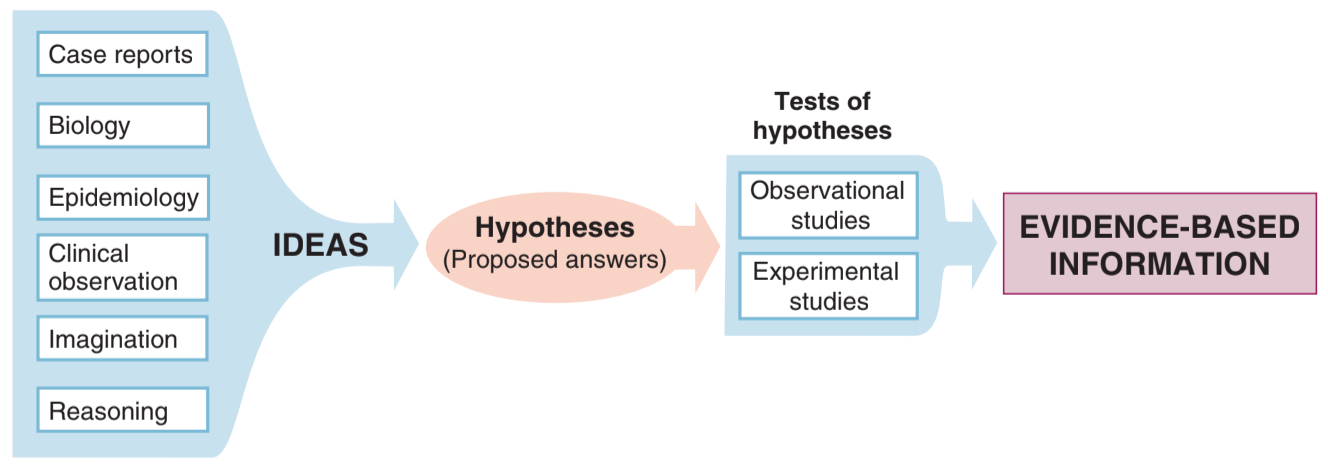
\includegraphics[width=1\linewidth]{figures/dieutri_01} 

}

\caption{Từ ý tưởng đến bằng chứng}\label{fig:unnamed-chunk-2}
\end{figure}

Ví dụ???

\hypertarget{cuxe1c-vux1ea5n-ux111ux1ec1-vux1ec1-ux111ux1ea1o-ux111ux1ee9c-khi-tiux1ebfn-huxe0nh-mux1ed9t-nghiuxean-cux1ee9u-luxe2m-suxe0ng-vux1ec1-ux111iux1ec1u-trux1ecb}{%
\section{Các vấn đề về đạo đức khi tiến hành một nghiên cứu lâm sàng về điều trị}\label{cuxe1c-vux1ea5n-ux111ux1ec1-vux1ec1-ux111ux1ea1o-ux111ux1ee9c-khi-tiux1ebfn-huxe0nh-mux1ed9t-nghiuxean-cux1ee9u-luxe2m-suxe0ng-vux1ec1-ux111iux1ec1u-trux1ecb}}

\begin{itemize}
\item
  Khi nào thì một nghiên cứu lâm sàng về điều trị là cần thiết và phù hợp?
\item
  Chọn nhóm chứng như thế nào là phù hợp?
\item
  Khi nào thì việc phân nhóm ngẫu nhiên bệnh nhân vào nhóm điều trị khác nhau là phù hợp?
\end{itemize}

``Equipoise'': không có lý do nào để tin rằng một phương pháp điều trị là tốt hơn điều trị còn lại. Ai quyết định? Như thế nào là tốt hơn?

\begin{itemize}
\tightlist
\item
  Các nguyên tắc về đạo đức khác

  \begin{itemize}
  \tightlist
  \item
    Informed consent: bệnh nhân cần được giải thích và hiểu rõ về quyền lợi và rủi ro khi tham gia nghiên cứu, tự nguyện và không bị ép buộc tham gia nghiên cứu\\
  \item
    Được quyền rút lui bất kỳ lúc nào
  \end{itemize}
\end{itemize}

\hypertarget{cuxe1c-cuxe2u-hux1ecfi-nghiuxean-cux1ee9u-liuxean-quan-ux111ux1ebfn-phux1b0ux1a1ng-phuxe1p-ux111iux1ec1u-trux1ecb}{%
\section{Các câu hỏi nghiên cứu liên quan đến phương pháp điều trị}\label{cuxe1c-cuxe2u-hux1ecfi-nghiuxean-cux1ee9u-liuxean-quan-ux111ux1ebfn-phux1b0ux1a1ng-phuxe1p-ux111iux1ec1u-trux1ecb}}

PICO

\hypertarget{duxe2n-sux1ed1-nghiuxean-cux1ee9u}{%
\subsection{Dân số nghiên cứu}\label{duxe2n-sux1ed1-nghiuxean-cux1ee9u}}

Để có bằng chứng trực tiếp và thuyết phục về hiệu quả của các phương pháp điều trị, các nghiên cứu lâm sàng cần được tiến hành trên người bệnh. Việc lựa chọn đối tượng nghiên cứu cụ thể được thể hiện qua các tiêu chuẩn chọn vào và loại ra cụ thể, và sẽ tuỳ theo mục đích của nghiên cứu.

Nếu mục tiêu chính của nghiên cứu là nhằm chứng minh hiệu lực

\hypertarget{ux111iux1ec1u-trux1ecb}{%
\subsection{Điều trị}\label{ux111iux1ec1u-trux1ecb}}

\hypertarget{nhuxf3m-so-suxe1nh}{%
\subsection{Nhóm so sánh}\label{nhuxf3m-so-suxe1nh}}

\hypertarget{kux1ebft-cuux1ed9c}{%
\subsection{Kết cuộc}\label{kux1ebft-cuux1ed9c}}

\hypertarget{cuxe1c-dux1ea1ng-nghiuxean-cux1ee9u-luxe2m-suxe0ng-giuxfap-ux111uxe1nh-giuxe1-mux1ed9t-phux1b0ux1a1ng-phuxe1p-ux111iux1ec1u-trux1ecb}{%
\section{Các dạng nghiên cứu lâm sàng giúp đánh giá một phương pháp điều trị}\label{cuxe1c-dux1ea1ng-nghiuxean-cux1ee9u-luxe2m-suxe0ng-giuxfap-ux111uxe1nh-giuxe1-mux1ed9t-phux1b0ux1a1ng-phuxe1p-ux111iux1ec1u-trux1ecb}}

\hypertarget{cuxe1ch-ux111ux1ecdc-vuxe0-ux111uxe1nh-giuxe1-mux1ed9t-nghiuxean-cux1ee9u-vux1ec1-ux111iux1ec1u-trux1ecb}{%
\section{Cách đọc và đánh giá một nghiên cứu về điều trị}\label{cuxe1ch-ux111ux1ecdc-vuxe0-ux111uxe1nh-giuxe1-mux1ed9t-nghiuxean-cux1ee9u-vux1ec1-ux111iux1ec1u-trux1ecb}}

\hypertarget{vuxed-dux1ee5-thux1ef1c-tux1ebf-nghiuxean-cux1ee9u-vux1ec1-ux111iux1ec1u-trux1ecb-covid-19}{%
\section{Ví dụ thực tế: nghiên cứu về điều trị COVID-19}\label{vuxed-dux1ee5-thux1ef1c-tux1ebf-nghiuxean-cux1ee9u-vux1ec1-ux111iux1ec1u-trux1ecb-covid-19}}

\hypertarget{buxe0i-tux1eadp}{%
\section{Bài tập}\label{buxe0i-tux1eadp}}

\hypertarget{ux111iux1ec1n-vuxe0o-chux1ed7-trux1ed1ng}{%
\subsection{Điền vào chỗ trống}\label{ux111iux1ec1n-vuxe0o-chux1ed7-trux1ed1ng}}

2 + 2 =

Gợi ý

See the documentation for \texttt{plot()} (\texttt{?plot})

Xem đáp án

4

\begin{Shaded}
\begin{Highlighting}[]
\DecValTok{4}
\end{Highlighting}
\end{Shaded}

\hypertarget{part-dux1ecbch-tux1ec5-hux1ecdc-thux1ef1c-ux111ux1ecba}{%
\part{DỊCH TỄ HỌC THỰC ĐỊA}\label{part-dux1ecbch-tux1ec5-hux1ecdc-thux1ef1c-ux111ux1ecba}}

\hypertarget{part-sinh-thux1ed1ng-kuxea-cux1a1-bux1ea3n}{%
\part{SINH THỐNG KÊ CƠ BẢN}\label{part-sinh-thux1ed1ng-kuxea-cux1a1-bux1ea3n}}

\hypertarget{stkcb_xacsuat}{%
\chapter{Kiến thức cơ bản về xác suất}\label{stkcb_xacsuat}}

\hypertarget{cuxe1c-khuxe1i-niux1ec7m-cux1a1-bux1ea3n}{%
\section{Các khái niệm cơ bản}\label{cuxe1c-khuxe1i-niux1ec7m-cux1a1-bux1ea3n}}

Các tính toán về xác suất bắt đầu với các \textbf{thử nghiệm (experiment)}. Mỗi thử nghiệm là một hoặc một chuỗi các hành động đưa đến kết quả. Các thử nghiệm này có thể được lặp đi lặp lại nhiều lần. Kết quả từ các thử nghiệm sẽ giúp tính toán các xác suất tương ứng.

Kết quả của một thử nghiệm được gọi là \textbf{kết cục (outcome)}. Một thử nghiệm có thể có nhiều kết cục khác nhau. Tuy nhiên, trong mỗi một lần thử nghiệm, chúng ta chỉ có thể quan sát được duy nhất một kết cục.

Tập hợp của tất cả các kết cục có thể có của một thử nghiệm được gọi là \textbf{không gian mẫu (sample space)}.

\textbf{Biến cố (event)} là một sự kiện bao gồm một hoặc một vài kết cuộc trong không gian mẫu. Do đó biến cố là một tập hợp con của không gian mẫu. Một biến cố được xem là xảy ra (occurred) nếu kết cục thực tế quan sát thấy có chứa trong biến cố đó.

\hypertarget{vuxed-dux1ee5-1-tung-mux1ed9t-ux111ux1ed3ng-xu-mux1ed9t-lux1ea7n-flip-a-coin-one-time}{%
\subsection{Ví dụ 1: Tung một đồng xu một lần (flip a coin one time)}\label{vuxed-dux1ee5-1-tung-mux1ed9t-ux111ux1ed3ng-xu-mux1ed9t-lux1ea7n-flip-a-coin-one-time}}

Ở đây, thử nghiệm là tung đồng xu một lần.

Các kết cục có thể có của thử nghiệm này là được mặt sấp (\(S\)) hoặc mặt ngửa (\(N\)).

Do đó, không gian mẫu sẽ là một tập hợp với 2 phần tử: \(S = \{\text{S},\text{N} \}\).

Trên không gian mẫu này có thể định nghĩa nhiều biến cố khác nhau:

\begin{itemize}
\tightlist
\item
  Biến cố được mặt ngửa: \(A = \{\text{N}\}\)
\item
  Biến cố được mặt sấp: \(B = \{\text{S}\}\)
\end{itemize}

Nếu thực hiện thử nghiệm và kết quả được mặt sấp, như vậy biến cố \(A\) đã xảy ra.

\begin{figure}

{\centering 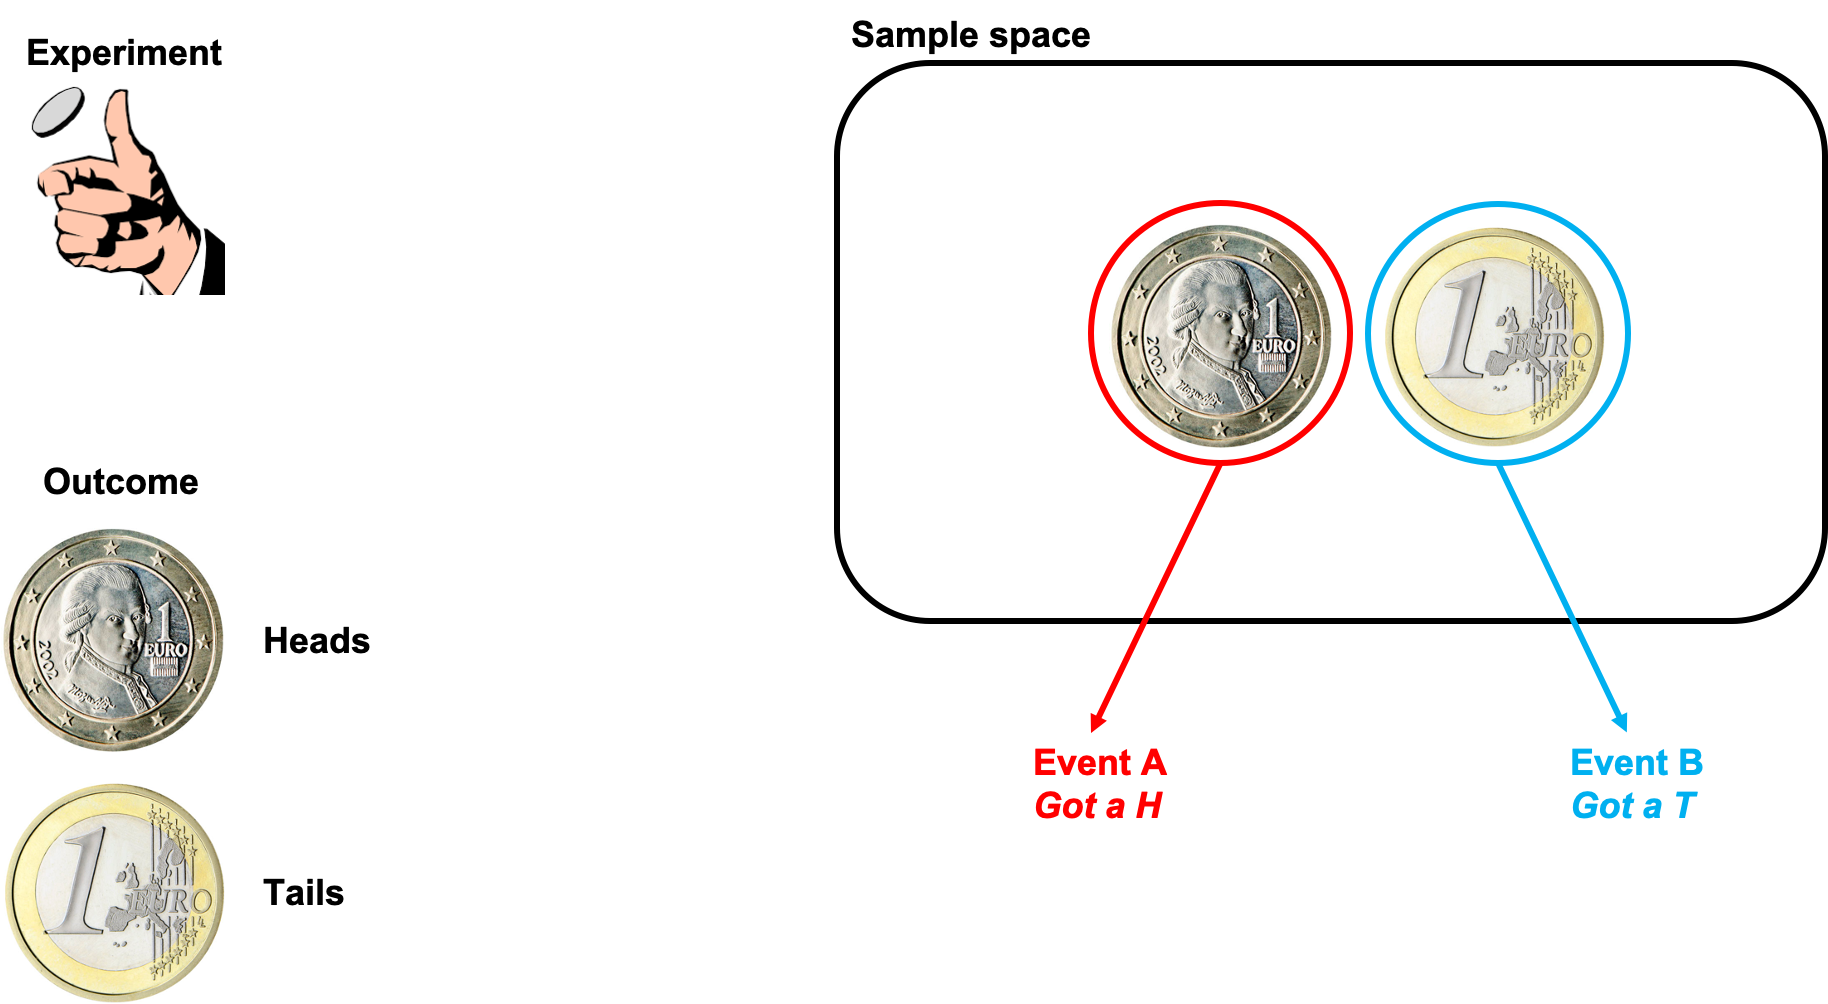
\includegraphics[width=1\linewidth]{figures/Picture01} 

}

\caption{Minh hoạ cho ví dụ 1}\label{fig:example1}
\end{figure}

\hypertarget{vuxed-dux1ee5-2-tung-mux1ed9t-ux111ux1ed3ng-xu-hai-lux1ea7n}{%
\subsection{Ví dụ 2: Tung một đồng xu hai lần}\label{vuxed-dux1ee5-2-tung-mux1ed9t-ux111ux1ed3ng-xu-hai-lux1ea7n}}

Ở đây, thử nghiệm là tung đồng xu hai lần.

Các kết cục có thể có của thử nghiệm này là được 2 mặt sấp (\(SS\)), hoặc 2 mặt ngửa (\(NN\)), hoặc ngửa rồi sấp (\(NS\)), hoặc sấp rồi ngửa (\(SN\)).

Do đó, không gian mẫu sẽ là một tập hợp với 4 phần tử: \(S = \{\text{SS},\text{NN},\text{NS},\text{SN}\}\).

Trên không gian mẫu này có thể định nghĩa nhiều biến cố khác nhau, ví dụ như:

\begin{itemize}
\tightlist
\item
  Biến cố được mặt ngửa đầu tiên: \(A = \{\text{NN},\text{NS}\}\)
\item
  Biến cố được mặt thứ hai là mặt ngửa: \(B = \{\text{NN},\text{SN}\}\)
\end{itemize}

Nếu thực hiện thử nghiệm và kết quả được 2 mặt ngửa, như vậy cả biến cố \(A\) và biến cố \(B\) đều đã xảy ra.

\begin{figure}

{\centering 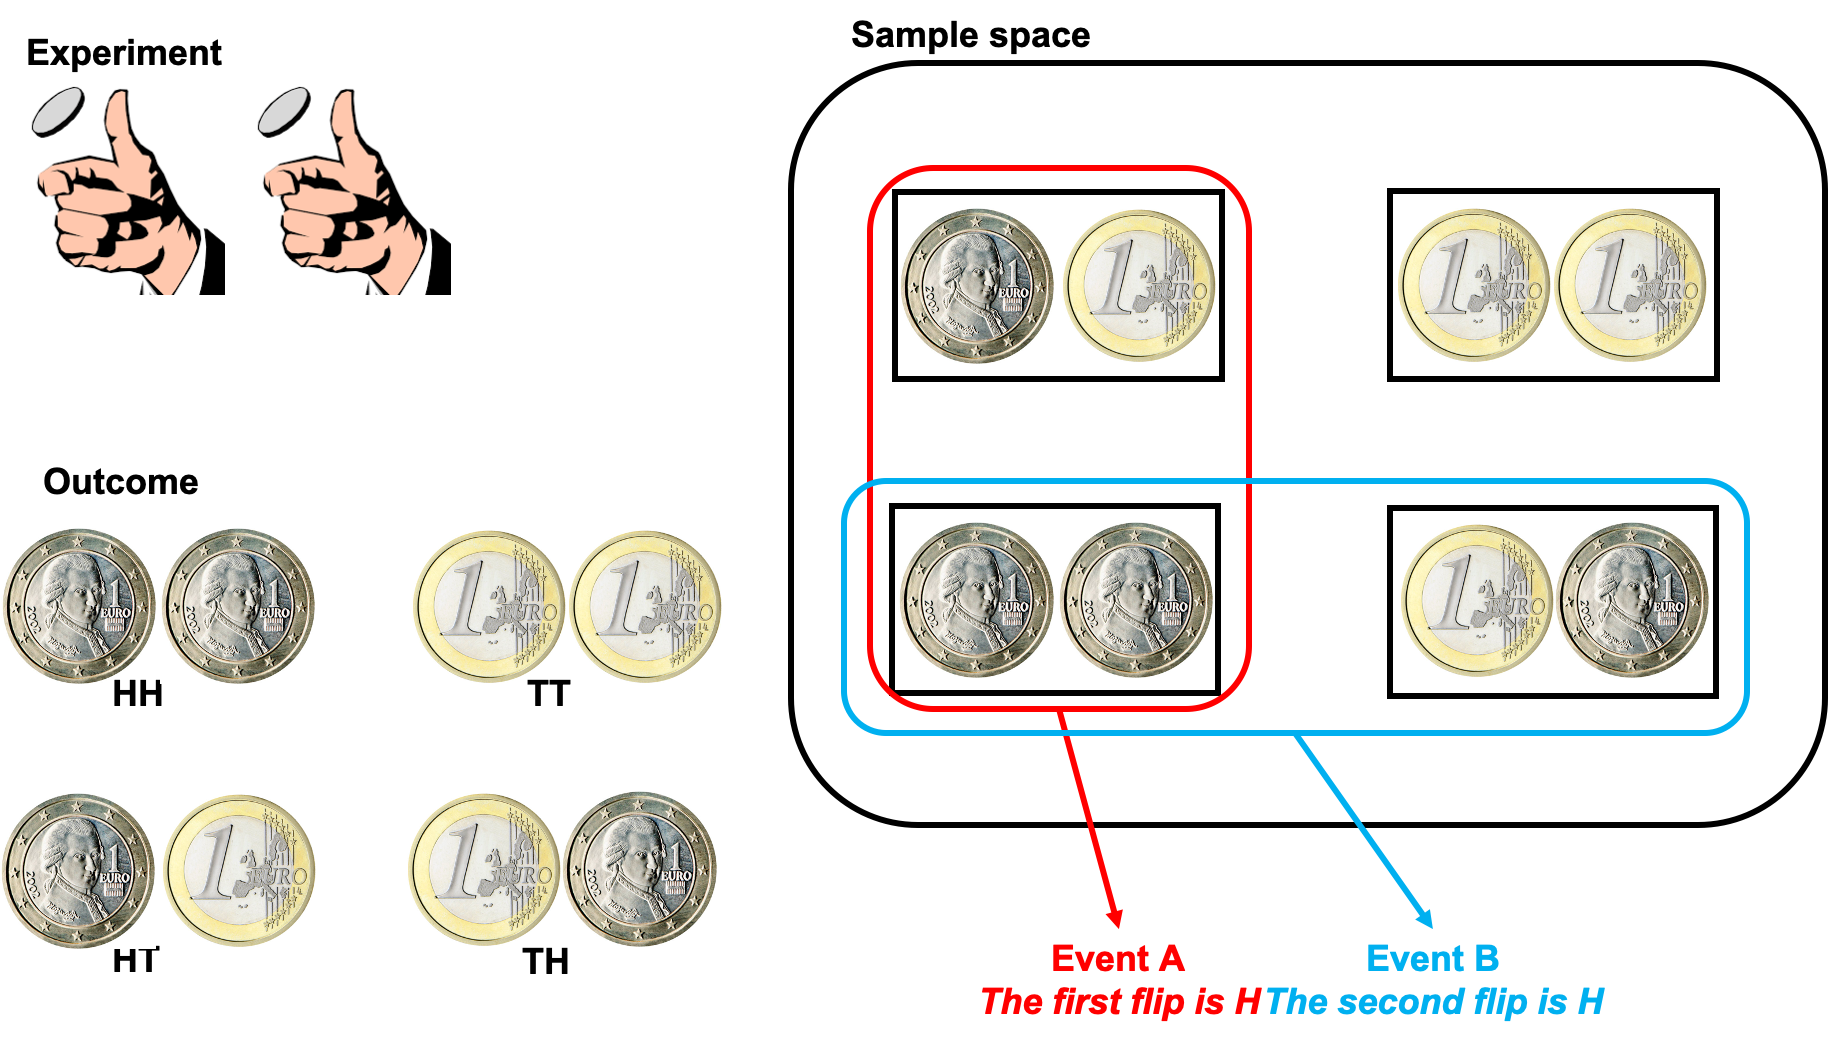
\includegraphics[width=1\linewidth]{figures/Picture02} 

}

\caption{Minh hoạ cho ví dụ 2}\label{fig:example2}
\end{figure}

\hypertarget{vuxed-dux1ee5-3-viuxeam-tux129nh-mux1ea1ch-phlebitis-sau-khi-sux1eed-dux1ee5ng-ux111ux1b0ux1eddng-truyux1ec1n-tux129nh-mux1ea1ch-ngoux1ea1i-biuxean-peripheral-intravenous-catheter}{%
\subsection{Ví dụ 3: viêm tĩnh mạch (phlebitis) sau khi sử dụng đường truyền tĩnh mạch ngoại biên (peripheral intravenous catheter)}\label{vuxed-dux1ee5-3-viuxeam-tux129nh-mux1ea1ch-phlebitis-sau-khi-sux1eed-dux1ee5ng-ux111ux1b0ux1eddng-truyux1ec1n-tux129nh-mux1ea1ch-ngoux1ea1i-biuxean-peripheral-intravenous-catheter}}

Ở đây, thử nghiệm là sử dụng đường truyền tĩnh mạch ngoại biên.

Các kết cục có thể có của thử nghiệm này là bị viêm tĩnh mạch (\(\text{VTM+}\)) hoặc không bị viêm tĩnh mạch (\(\text{VTM-}\)).

Do đó, không gian mẫu sẽ là một tập hợp với 2 thành phần: \(S = \{\text{VTM+},\text{VTM-}\}\).

Trên không gian mẫu này có thể định nghĩa biến cố \(A\) là biến cố xảy ra viêm tĩnh mạch: \(A = \{VTM+\}\)

Nếu một bệnh nhân được sử dụng đường truyền tĩnh mạch và sau đó bị viêm tĩnh mạch thì ta nói rằng biến cố \(A\) đã xảy ra.

\hypertarget{luxfd-thuyux1ebft-vux1ec1-tux1eadp-hux1ee3p-sets}{%
\subsection{Lý thuyết về tập hợp (sets)}\label{luxfd-thuyux1ebft-vux1ec1-tux1eadp-hux1ee3p-sets}}

Với \(A\) và \(B\) là 2 biến cố được định nghĩa trên cùng không gian mẫu \(S\)

\begin{itemize}
\tightlist
\item
  Hợp (union) của \(A\) và \(B\) (\(A \cup B\)) là một biến cố xảy ra khi và chỉ khi \(A\) hay \(B\) xảy ra.
\item
  Giao (intersection) của \(A\) và \(B\) (\(A \cap B\)) là một biến cố xảy ra khi và chỉ khi \(A\) và \(B\) xảy ra.
\item
  Phần bù (complement) của \(A\) (\(A^c\)) là một biến cố xảy ra khi và chỉ khi \(A\) không xảy ra.
\end{itemize}

Quay trở lại ví dụ 2:

\begin{itemize}
\tightlist
\item
  Gọi \(C\) là biến cố có ít nhất 1 mặt ngửa: \(C = A \cup B = \{\text{NN},\text{NS},\text{SN}\}\)
\item
  Gọi \(D\) là biến cố cả 2 mặt đều là mặt ngửa: \(D = A \cap B = \{\text{NN}\}\)
\item
  Gọi \(E\) là biến cố có mặt sấp đầu tiên: \(E = A^c = \{\text{SN},\text{SS}\}\)
\end{itemize}

\begin{figure}

{\centering 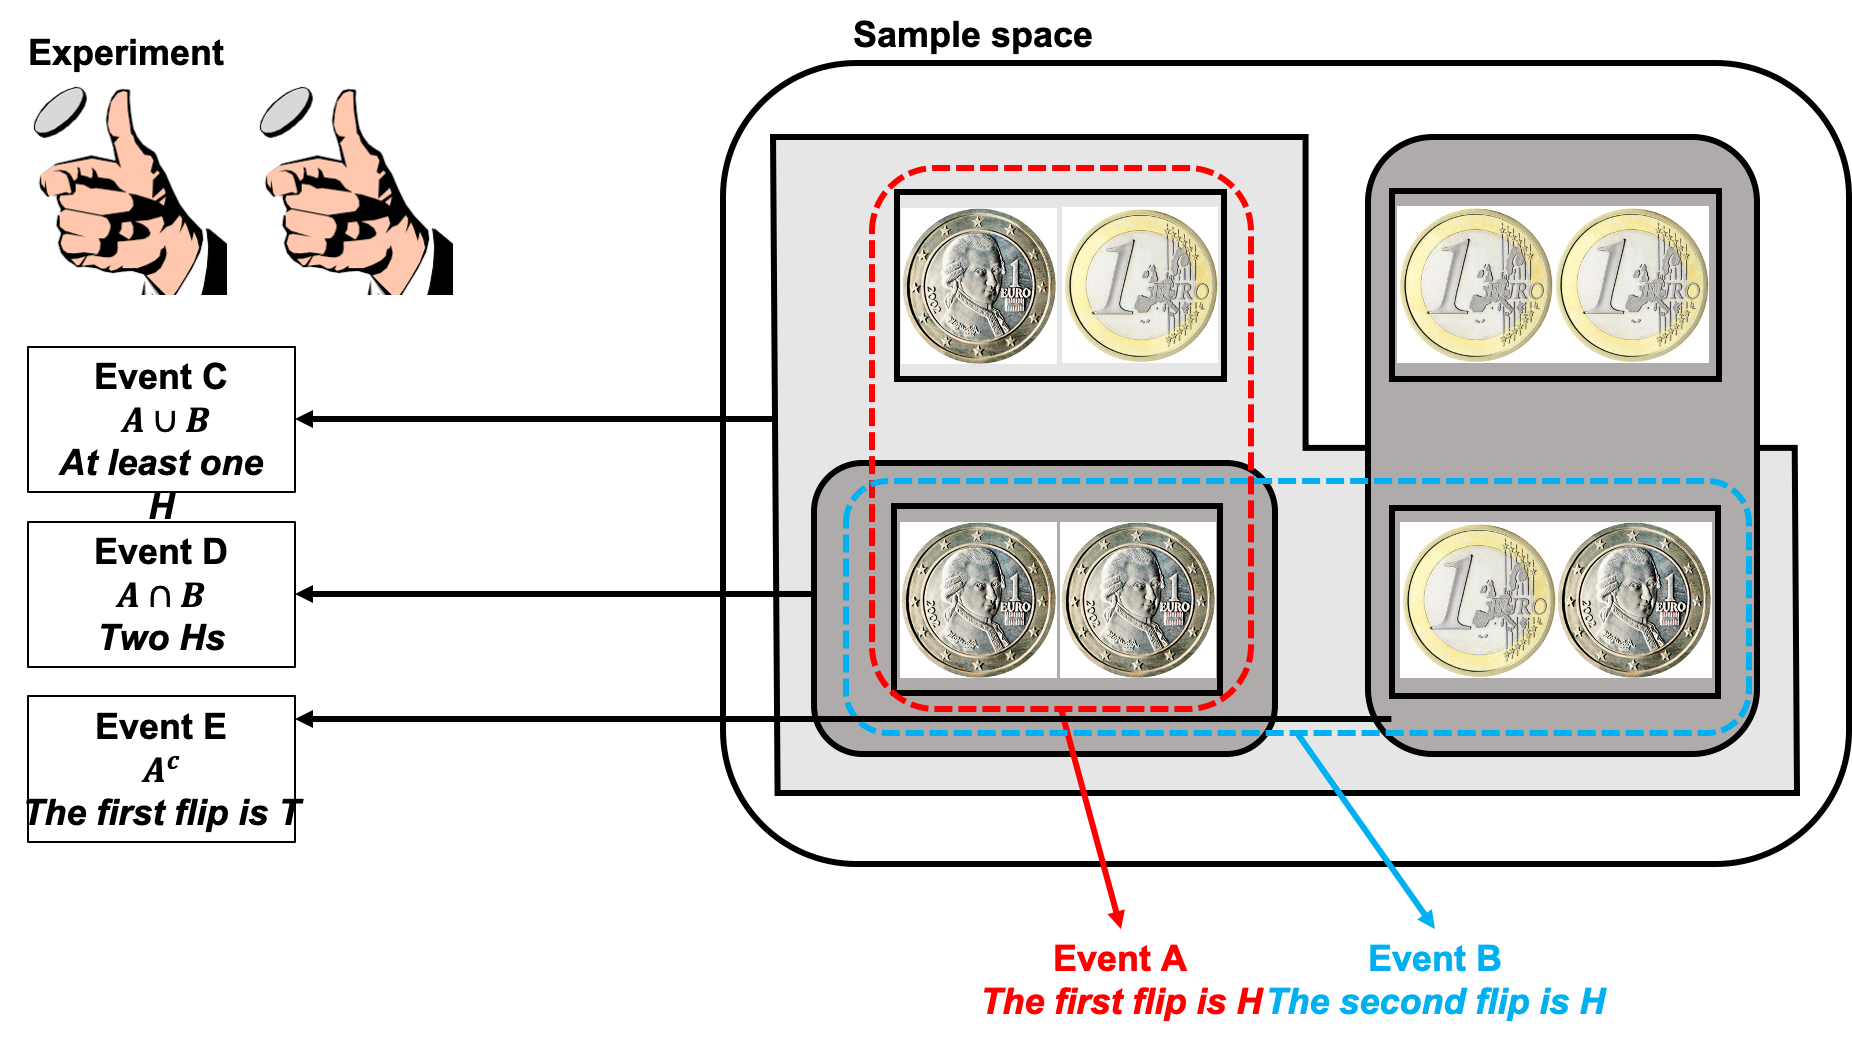
\includegraphics[width=1\linewidth]{figures/Picture03} 

}

\caption{Minh hoạ cho lý thuyết tập hợp}\label{fig:example3}
\end{figure}

\hypertarget{ux111ux1ecbnh-nghux129a-xuxe1c-suux1ea5t-probability}{%
\section{Định nghĩa xác suất (probability)}\label{ux111ux1ecbnh-nghux129a-xuxe1c-suux1ea5t-probability}}

\hypertarget{ux111ux1ecbnh-nghux129a-ux111ux1a1n-giux1ea3n-vux1ec1-xuxe1c-suux1ea5t-naive-definition-of-probability}{%
\subsection{Định nghĩa đơn giản về xác suất (naive definition of probability)}\label{ux111ux1ecbnh-nghux129a-ux111ux1a1n-giux1ea3n-vux1ec1-xuxe1c-suux1ea5t-naive-definition-of-probability}}

Gọi \(A\) là một biến cố trong một thử nghiệm với không gian mẫu \(S\).

Xác suất xảy ra của \(A\) (định nghĩa đơn giản) là:

\[
P(A) = \frac{\text{Size of A}}{\text{Size of S}} = \frac{\text{Số lượng kết cục của A}}{\text{Tổng số kết cục trong S}}
\]

Trong ví dụ 2:

\begin{itemize}
\tightlist
\item
  \(P(A) = \frac{2}{4} = 0.5\)
\item
  \(P(B) = \frac{2}{4} = 0.5\)
\item
  \(P(C) = \frac{3}{4} = 0.75\)
\item
  \(P(D) = \frac{1}{4} = 0.25\)
\item
  \(P(E) = \frac{2}{4} = 0.5\)
\end{itemize}

\hypertarget{tuxednh-xuxe1c-suux1ea5t-theo-quy-tux1eafc-nhuxe2n-multiplication-rule}{%
\subsection{Tính xác suất theo quy tắc nhân (multiplication rule)}\label{tuxednh-xuxe1c-suux1ea5t-theo-quy-tux1eafc-nhuxe2n-multiplication-rule}}

Để tính xác suất (theo định nghĩa đơn giản) của biến cố \(A\), chúng ta cần đếm được số phần tử của \(A\) và số phần tử của \(B\). Trong nhiều trường hợp, những số lượng này rất lớn và do đó, không thể đếm trực tiếp theo cách thông thường được. Một cách đếm nhanh hơn là sử dụng \textbf{quy tắc nhân (multiplication rule)}:

\begin{quote}
Thực hiện một thử nghiệm phức tạp, kết hợp hai thử nghiệm \(A\) và \(B\). Giả sử thử nghiệm \(A\) có thể có \(a\) kết cục; và ứng với mỗi kết cục của \(A\), thử nghiệm \(B\) có \(b\) kết cục. Khi đó thử nghiệm phức tạp kết hợp \(A\) và \(B\) có thể có \(a \times b\) kết cục.
\end{quote}

\hypertarget{vuxed-dux1ee5-4-chux1ea1y-thi}{%
\subsubsection{Ví dụ 4: Chạy thi}\label{vuxed-dux1ee5-4-chux1ea1y-thi}}

\begin{quote}
Có 10 người tham gia một cuộc thi chạy. Giả định rằng không có trường hợp đồng hạng và cả 10 người đều hoàn thành đường đua của mình. Khi đó luôn xác định được người xếp hạng nhất, nhì, ba. Có tất cả bao nhiêu cách chọn ra được người xếp hạng nhất, nhì, ba?
\end{quote}

Có tất cả 10 cách chọn người xếp hạng nhất.

Sau khi chọn được người xếp hạng nhất, có 9 cách chọn người xếp hạng nhì.

Sau khi đã chọn được người xếp hạng nhất và hạng nhì, có 8 cách chọn người xếp hạng ba.

Như vậy có tất cả \(10 \times 9 \times 8 = 720\) cách chọn ra được người xếp hạng nhất, nhì, ba.

\hypertarget{ux111ux1ecbnh-luxfd-vux1ec1-chux1ecdn-mux1eabu-lux1eb7p-lux1ea1i-sampling-with-replacement}{%
\subsubsection{Định lý về chọn mẫu lặp lại (sampling with replacement)}\label{ux111ux1ecbnh-luxfd-vux1ec1-chux1ecdn-mux1eabu-lux1eb7p-lux1ea1i-sampling-with-replacement}}

\begin{quote}
Có \(n\) đối tượng và cần lần lượt chọn ra \(k\) phần tử từ các đối tượng này, theo kiểu \textbf{lặp lại} (một đối tượng đã được chọn vẫn có thể tiếp tục được chọn trong lần chọn tiếp theo). Khi đó sẽ có tất cả \(n^k\) cách chọn (có tính đến thứ tự).
\end{quote}

\hypertarget{ux111ux1ecbnh-luxfd-vux1ec1-chux1ecdn-mux1eabu-khuxf4ng-lux1eb7p-lux1ea1i-sampling-without-replacement}{%
\subsubsection{Định lý về chọn mẫu không lặp lại (sampling without replacement)}\label{ux111ux1ecbnh-luxfd-vux1ec1-chux1ecdn-mux1eabu-khuxf4ng-lux1eb7p-lux1ea1i-sampling-without-replacement}}

\begin{quote}
Có \(n\) đối tượng và cần lần lượt chọn ra \(k\) phần tử từ các đối tượng này, theo kiểu \textbf{không lặp lại} (một đối tượng đã được chọn thì không thể được chọn trong lần chọn tiếp theo). Khi đó sẽ có tất cả \(n \times (n-1) \ldots (n-k+1)\) cách chọn (có tính đến thứ tự), với \(k \leq n\). Khi \(k=n\), số cách chọn là \(n \times (n-1) \ldots 1 = n!\)
\end{quote}

\hypertarget{vuxed-dux1ee5-5-the-last-banana}{%
\subsection{Ví dụ 5: the last banana}\label{vuxed-dux1ee5-5-the-last-banana}}

\begin{quote}
Minh và Lan bị lạc trên hoang đảo. Đến ngày hôm nay thức ăn chỉ còn lại một quả chuối. Để phân định ai sẽ được ăn quả chuối, Minh và Lan quyết định cầu may bằng việc tung xúc sắc. Sau khi mỗi người tung xúc sắc của mình, điểm xúc sắc của hai người sẽ được so với nhau để xác định điểm cao nhất. Nếu điểm cao nhất là từ 1 đến 4 thì Minh thắng và được ăn quả chuối; nhưng nếu điểm cao nhất là 5 hay 6 thì Lan sẽ thắng. Hãy xác định xem giữa Minh và Lan thì ai có xác suất thắng cao hơn?
\end{quote}

Trong ví dụ này thử nghiệm là tung hai xúc sắc.

Khi tung một xúc sắc có thể có 6 kết cục khác nhau. Theo quy tắc nhân, khi tung hai xúc sắc sẽ có tất cả \(6 \times 6 = 36\) kết cục khác nhau.

Gọi \(A\) là biến cố điểm cao nhất trong một lần tung 2 xúc sắc là từ 1 đến 4.

Gọi \(B\) là biến cố điểm cao nhất trong một lần tung 2 xúc sắc là từ 5 đến 6.

Không gian mẫu, điểm cao nhất trong từng kết cục và khả năng xuất hiện của biến cố \(A\) và \(B\) trong không gian mẫu được trình bày ở hình sau:

\begin{figure}

{\centering 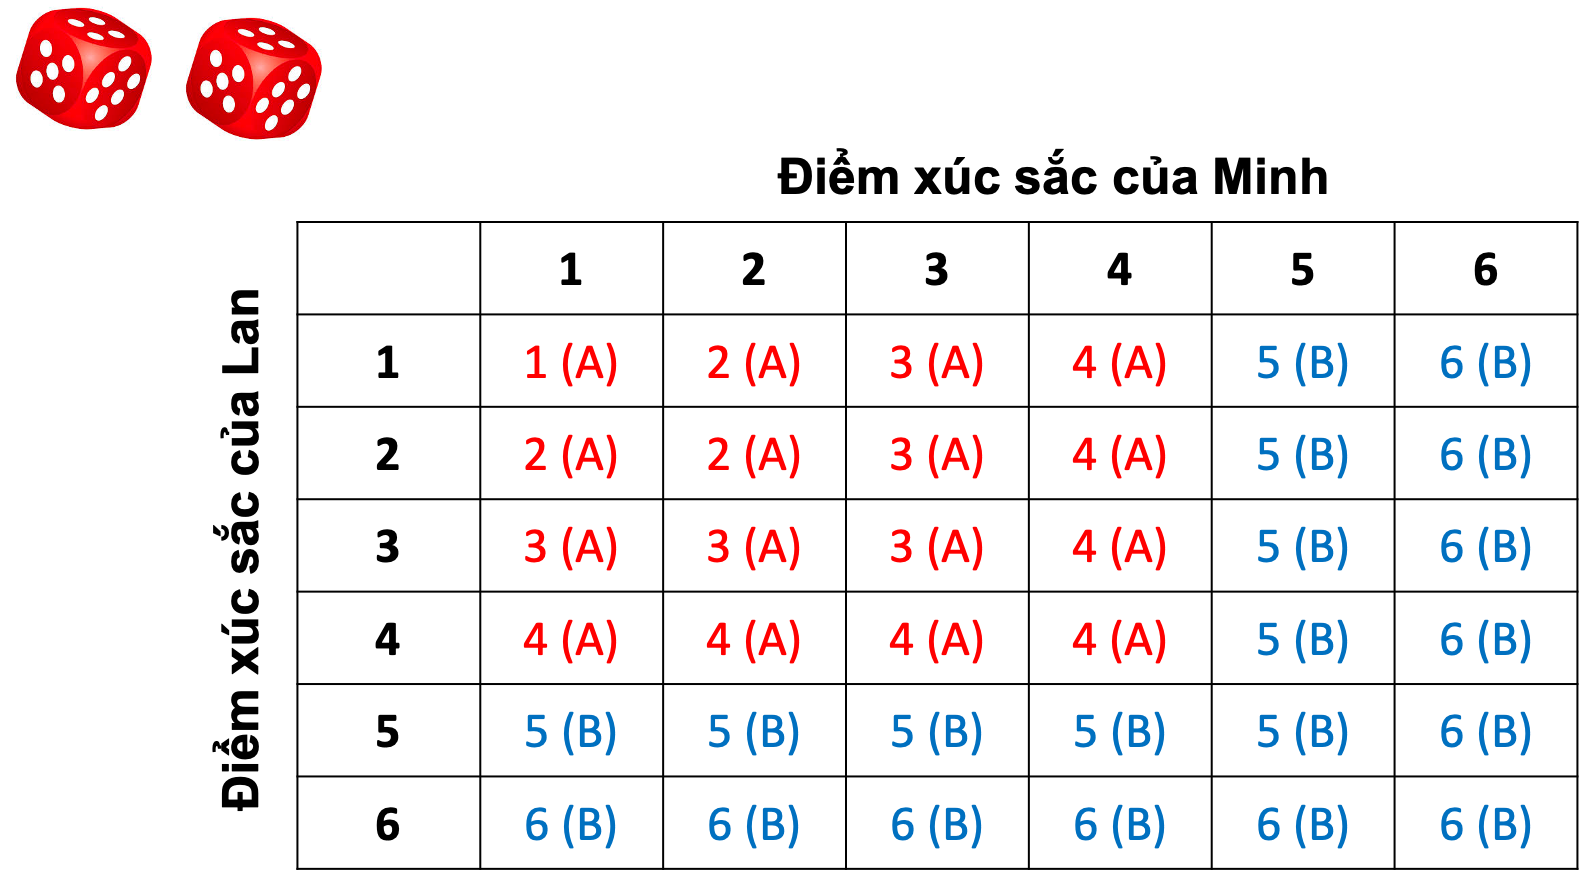
\includegraphics[width=1\linewidth]{figures/Picture04} 

}

\caption{Minh hoạ cho ví dụ 5}\label{fig:example5}
\end{figure}

Như vậy xác suất \(A\) xảy ra là \(P(A) = \frac{16}{36} = 0.44\), còn xác suất \(B\) xảy ra là \(P(B) = \frac{20}{36} = 0.56\)

Như vậy Lan có xác suất thắng cao hơn.

Link Youtube cho ví dụ này: \url{https://youtu.be/Kgudt4PXs28}

\hypertarget{hux1ea1n-chux1ebf-cux1ee7a-ux111ux1ecbnh-nghux129a-ux111ux1a1n-giux1ea3n-vux1ec1-xuxe1c-suux1ea5t}{%
\subsection{Hạn chế của định nghĩa đơn giản về xác suất}\label{hux1ea1n-chux1ebf-cux1ee7a-ux111ux1ecbnh-nghux129a-ux111ux1a1n-giux1ea3n-vux1ec1-xuxe1c-suux1ea5t}}

Định nghĩa đơn giản trên về xác suất có hai hạn chế chính:

\begin{itemize}
\tightlist
\item
  Không gian mẫu \(S\) phải hữu hạn (finite sample space)
\item
  Các kết cục có khả năng xảy ra như nhau (equally likely outcome)
\end{itemize}

\hypertarget{ux111ux1ecbnh-nghux129a-ux111ux1ea7y-ux111ux1ee7-vux1ec1-xuxe1c-suux1ea5t}{%
\subsection{Định nghĩa đầy đủ về xác suất}\label{ux111ux1ecbnh-nghux129a-ux111ux1ea7y-ux111ux1ee7-vux1ec1-xuxe1c-suux1ea5t}}

Một không gian xác suất (probability space) bao gồm một không gian mẫu \(S\) và một hàm số xác suất \(P\), trong đó hàm số xác suất \(P\) sẽ gán một số thực từ 0 đến 1 cho từng biến cố \(A\) trong \(S\). Hàm số \(P\) phải thoả mãn các tiên đề sau:

\begin{itemize}
\tightlist
\item
  \(P(\emptyset) = 0\) (xác suất của tập hợp rỗng bằng 0)
\item
  \(P(S) = 1\) (xác suất của không gian mẫu bằng 1)
\item
  Nếu \(A_1,A_2,\dots\) là các biến cố xung khắc (mutually exclusive or disjoint), thì: \(P(\bigcup\limits_{j=1}^{\infty} A_{j}) = \Sigma_{j=1}^{\infty}P(A_{j})\)
\end{itemize}

\hypertarget{cuxe1c-tuxednh-chux1ea5t-cux1ee7a-xuxe1c-suux1ea5t}{%
\subsubsection{Các tính chất của xác suất}\label{cuxe1c-tuxednh-chux1ea5t-cux1ee7a-xuxe1c-suux1ea5t}}

Với các biến cố \(A\) và \(B\) bất kỳ:

\begin{itemize}
\tightlist
\item
  \(P(A^c) = 1 - P(A)\)
\item
  Nếu \(A\) là tập hợp con của \(B\) (\(A \subseteq\) B) thì \(P(A) \leq P(B)\)
\item
  \(P(A \cup B) = P(A) + P(B) - P(A \cap B)\)
\end{itemize}

Định nghĩa và tính chất của xác suất được tóm tắt trong hình sau:

\begin{figure}

{\centering 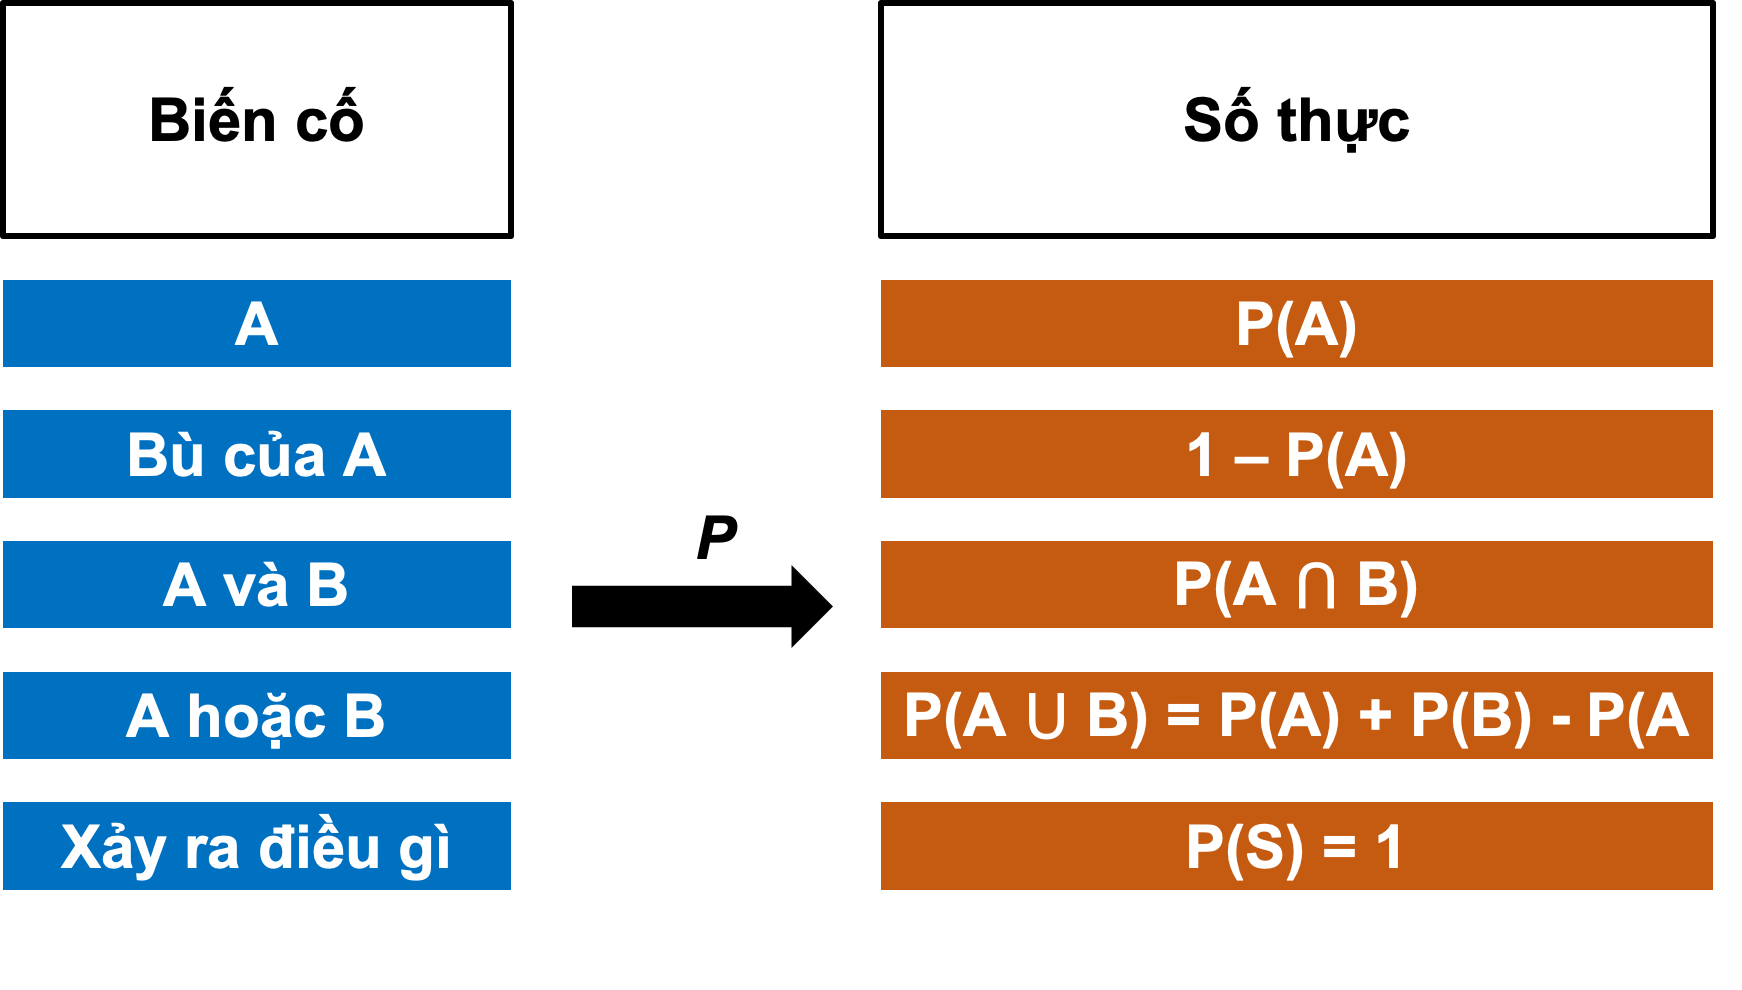
\includegraphics[width=1\linewidth]{figures/Picture05} 

}

\caption{Định nghĩa và tính chất của xác suất}\label{fig:generaldefinition}
\end{figure}

\hypertarget{diux1ec5n-giux1ea3i-uxfd-nghux129a-cux1ee7a-xuxe1c-suux1ea5t}{%
\subsection{Diễn giải ý nghĩa của xác suất}\label{diux1ec5n-giux1ea3i-uxfd-nghux129a-cux1ee7a-xuxe1c-suux1ea5t}}

\hypertarget{theo-trux1b0ux1eddng-phuxe1i-frequentist}{%
\subsubsection{Theo trường phái frequentist}\label{theo-trux1b0ux1eddng-phuxe1i-frequentist}}

Xác suất của một biến cố thể hiện tần số xuất hiện của biến cố đó khi lặp lại thử nghiệm nhiều lần. Ví dụ, xác suất được mặt ngửa khi tung một đồng xu bằng 50\%, nghĩa là nếu tung đồng xu rất nhiều lần, mặt ngửa sẽ xuất hiện trong khoảng 50\% số lần tung đó.

\hypertarget{theo-trux1b0ux1eddng-phuxe1i-bayesian}{%
\subsubsection{Theo trường phái Bayesian}\label{theo-trux1b0ux1eddng-phuxe1i-bayesian}}

Xác suất của một biến cố phản ánh mức độ tin tưởng vào sự xuất hiện của biến cố đó, kể cả khi không thể lặp lại thử nghiệm.

\hypertarget{xuxe1c-suux1ea5t-cuxf3-ux111iux1ec1u-kiux1ec7n}{%
\section{Xác suất có điều kiện}\label{xuxe1c-suux1ea5t-cuxf3-ux111iux1ec1u-kiux1ec7n}}

\hypertarget{ux111ux1ecbnh-nghux129a-xuxe1c-suux1ea5t-cuxf3-ux111iux1ec1u-kiux1ec7n}{%
\subsection{Định nghĩa xác suất có điều kiện}\label{ux111ux1ecbnh-nghux129a-xuxe1c-suux1ea5t-cuxf3-ux111iux1ec1u-kiux1ec7n}}

Nếu \(A\) và \(B\) là các biến cố với \(P(B) > 0\), xác suất của \(A\) khi biết \(B\) (\(P(A | B)\)) được tính bằng công thức

\[
P(A|B) = \frac{P(A \cap B)}{P(B)}
\]
\#\#\#\# Định lí về xác suất phần giao của hai biến cố

Với các biến cố \(A\) và \(B\) có xác suất \(>0\) bất kỳ:

\[
P(A \cap B) = P(B) \times P(A|B) = P(A) \times P(B|A)
\]

\hypertarget{ux111ux1ecbnh-luxed-bayes-bayes-rule}{%
\subsection{Định lí Bayes (Bayes' rule)}\label{ux111ux1ecbnh-luxed-bayes-bayes-rule}}

Với các biến cố \(A\) và \(B\) bất kỳ và \(P(B) > 0\):

\[
P(A|B) = \frac{P(B|A)P(A)}{P(B)}
\]
\(P(A)\) được gọi là \textbf{xác suất tiền nghiệm (prior probability)} của \(A\), và \(P(A|B)\) được gọi là xác suất hậu nghiệm (posterior probability) của \(A\) sau khi biết \(B\) đã xảy ra.

\hypertarget{luux1eadt-xuxe1c-suux1ea5t-touxe0n-phux1ea7n-law-of-total-probability}{%
\subsection{Luật xác suất toàn phần (law of total probability)}\label{luux1eadt-xuxe1c-suux1ea5t-touxe0n-phux1ea7n-law-of-total-probability}}

Gọi \(A_1,\ldots,A_n\) là các phần của không gian mẫu \(S\) (nghĩa là \(A_1,\ldots,A_n\) xung khắc với nhau, và hợp của chúng là \(S\)) và xác suất của các phần này đều \(>0\) (\(P(A_i) > 0\) với mọi \(i\))

\[
P(B) = \Sigma^n_{i = 1}P(B|A_i)P(A_i)
\]

Nói cách khác, để tính xác suất không điều kiện của \(B\), cần chia không gian mẫu \(S\) thành các phần không trùng lắp \(A_i\), sau đó tính xác suất có điều kiện của \(B\) trong từng phần, cuối cùng lấy tổng các tích số của xác suất có điều kiện đó với xác suất của từng phần.

\hypertarget{sux1ef1-ux111ux1ed9c-lux1eadp-cux1ee7a-cuxe1c-biux1ebfn-cux1ed1-independence-of-events}{%
\subsection{Sự độc lập của các biến cố (Independence of events)}\label{sux1ef1-ux111ux1ed9c-lux1eadp-cux1ee7a-cuxe1c-biux1ebfn-cux1ed1-independence-of-events}}

Hai biến cố \(A\) và \(B\) độc lập với nhau nếu

\[
P(A \cap B) = P(A) \times P(B)
\]
nói cách khác

\[
P(A|B) = P(A)
\]

Lưu ý, \textbf{độc lập (independence)} khác với \textbf{xung khắc (mutually exclusive/disjoint)}. Khi \(A\) và \(B\) xung khắc với nhau, chúng không độc lập với nhau, trừ khi \(P(A) = 0\) hay \(P(B) = 0\) (vì khi biết \(A\) xảy ra sẽ dễ dàng suy ra \(B\) không xảy ra).

\hypertarget{biux1ebfn-sux1ed1-ngux1eabu-nhiuxean-random-variables}{%
\section{Biến số ngẫu nhiên (Random variables)}\label{biux1ebfn-sux1ed1-ngux1eabu-nhiuxean-random-variables}}

\begin{quote}
Cho một thử nghiệm với không gian mẫu \(S\), một \textbf{biến số ngẫu nhiên} là một hàm số kết nối từ không gian mẫu \(S\) sang tập hợp số thực \(R\)
\end{quote}

Nói cách khác, biến số ngẫu nhiên \(X\) gán một giá trị \(X(s)\) cho mỗi kết cục \(s\) của thử nghiệm.

\hypertarget{vuxed-dux1ee5}{%
\subsection{Ví dụ:}\label{vuxed-dux1ee5}}

Quay trở lại với thử nghiệm tung 2 đồng xu.

Không gian mẫu bao gồm 4 kết cục: \(S = \{SS, NN, SN, NS\}\)

Dưới đây là một số biến số ngẫu nhiên có thể được định nghĩa trên không gian mẫu này:

\begin{itemize}
\item
  \(X\) là số mặt ngửa. Đây là một biến số ngẫu nhiên với 3 giá trị có thể có: 0, 1, 2. Biến số này gán 2 cho kết cục \(NN\) (\(X(NN) = 2\)), 1 cho kết cục \(NS\) hay \(SN\) (\(X(NS) = X(SN) = 1\)) và 0 cho kết cục \(SS\) (\(X(SS) = 0\))
\item
  \(Y\) là số mặt sấp. Có thể định nghĩa biến số ngẫu nhiên này bằng: \(Y(s) = 2 - X(s)\)
\item
  \(I = 1\) nếu được mặt ngửa đầu tiên và \(I = 0\) trong những trường hợp khác. Đây là một biến số ngẫu nhiên với 2 giá trị: 0, 1. Biến số này gán 1 cho kết cục \(NN\) hay \(NS\) (\(I(NN) = I(NS) = 1\)), và gán 0 cho kết cục \(SN\) hay \(SS\) (\(I(SN) = I(SS) = 0\))
\end{itemize}

\begin{figure}

{\centering 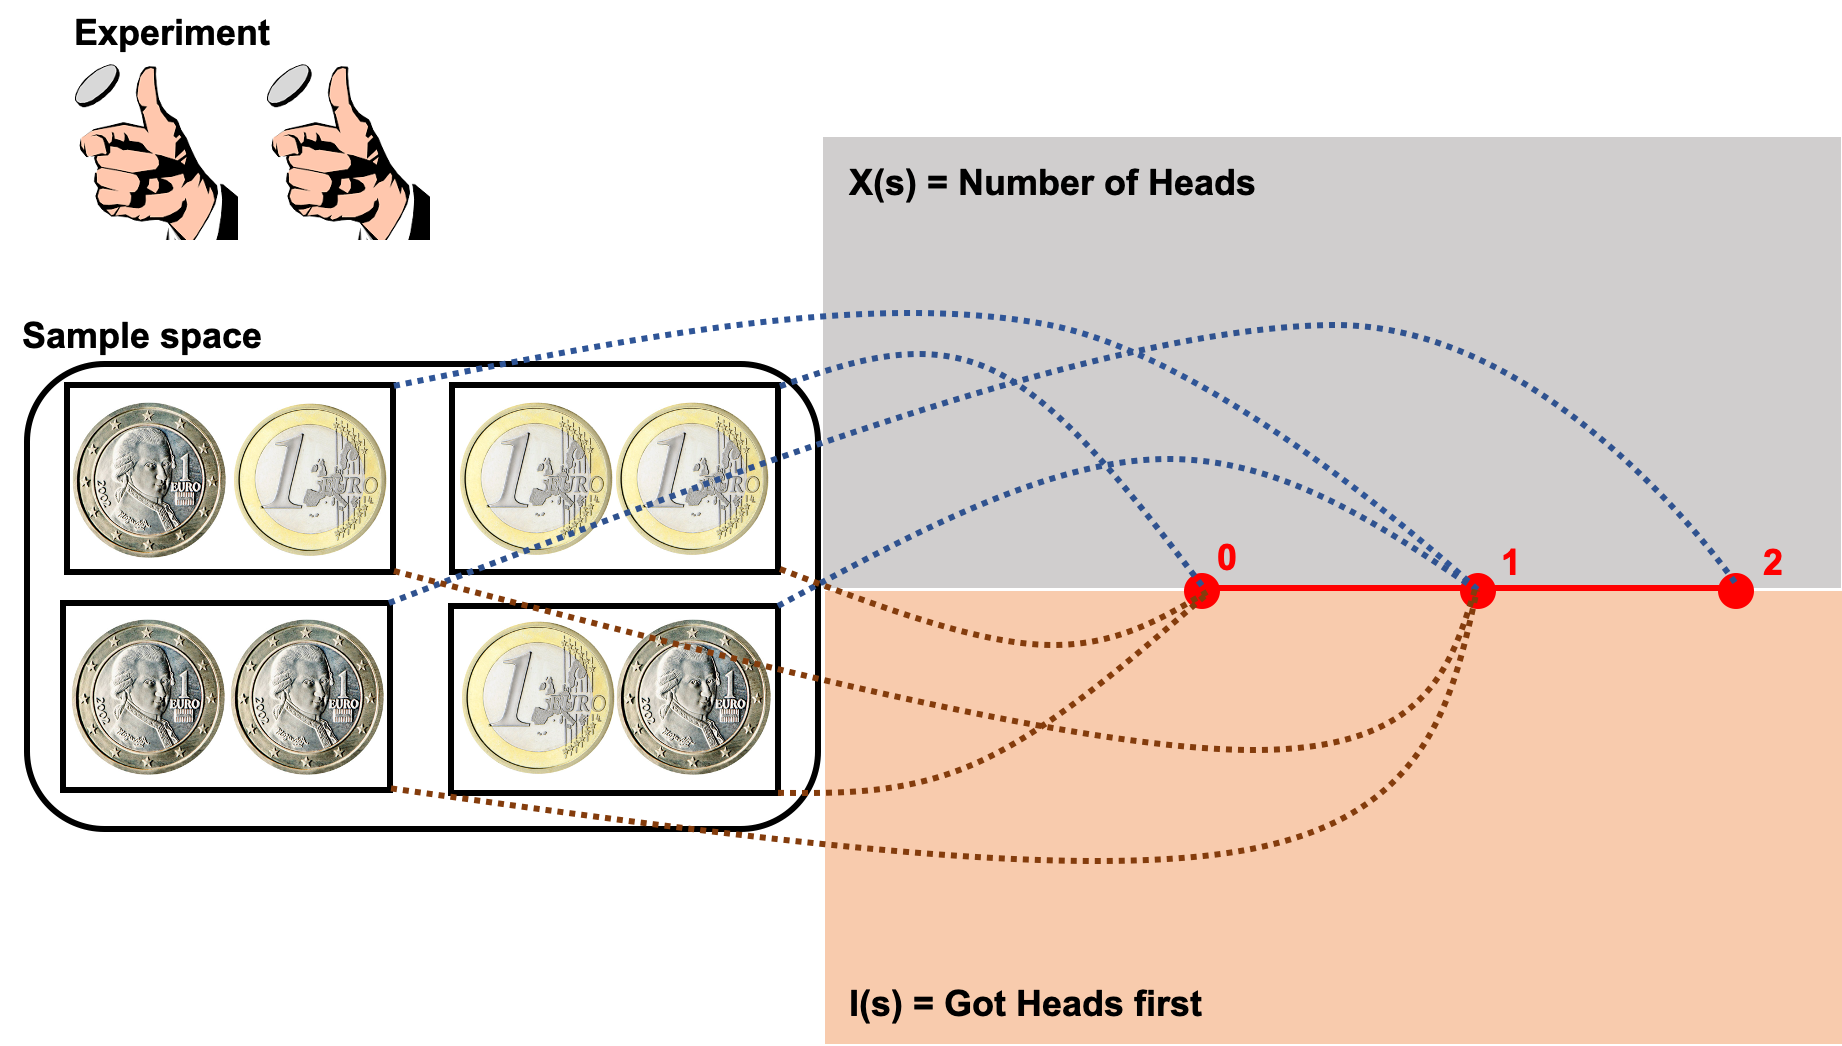
\includegraphics[width=1\linewidth]{figures/Picture06} 

}

\caption{Minh hoạ cho biến số ngẫu nhiên}\label{fig:unnamed-chunk-4}
\end{figure}

\hypertarget{loux1ea1i-biux1ebfn-sux1ed1-ngux1eabu-nhiuxean}{%
\subsection{Loại biến số ngẫu nhiên}\label{loux1ea1i-biux1ebfn-sux1ed1-ngux1eabu-nhiuxean}}

Có hai loại biến số ngẫu nhiên: \textbf{biến số ngẫu nhiên rời rạc (discrete random variables)} và \textbf{biến số ngẫu nhiên liên tục (continuous random variables)}.

\hypertarget{biux1ebfn-sux1ed1-ngux1eabu-nhiuxean-rux1eddi-rux1ea1c-discrete-random-variables}{%
\subsubsection{Biến số ngẫu nhiên rời rạc (discrete random variables)}\label{biux1ebfn-sux1ed1-ngux1eabu-nhiuxean-rux1eddi-rux1ea1c-discrete-random-variables}}

\begin{quote}
Một biến số ngẫu nhiên X được xem là rời rạc nếu tập hợp các giá trị có thể có của X là một tập hợp hữu hạn hoặc vô hạn nhưng đếm được.
\end{quote}

\begin{quote}
Một biến số ngẫu nhiên X được xem là liên tục nếu X có thể có bất kỳ giá trị nào trong một khoảng trên trục số
\end{quote}

\hypertarget{phuxe2n-phux1ed1i-xuxe1c-suux1ea5t-probability-distribution}{%
\section{Phân phối xác suất (Probability distribution)}\label{phuxe2n-phux1ed1i-xuxe1c-suux1ea5t-probability-distribution}}

Phân phối của một biến số ngẫu nhiên mô tả xác suất của mọi biến cố liên quan đến biến số ngẫu nhiên.

\hypertarget{phuxe2n-phux1ed1i-cux1ee7a-biux1ebfn-sux1ed1-ngux1eabu-nhiuxean-rux1eddi-rux1ea1c}{%
\subsection{Phân phối của biến số ngẫu nhiên rời rạc}\label{phuxe2n-phux1ed1i-cux1ee7a-biux1ebfn-sux1ed1-ngux1eabu-nhiuxean-rux1eddi-rux1ea1c}}

\hypertarget{huxe0m-khux1ed1i-xuxe1c-suux1ea5t-probability-mass-function-pmf}{%
\subsubsection{Hàm khối xác suất (Probability mass function, PMF)}\label{huxe0m-khux1ed1i-xuxe1c-suux1ea5t-probability-mass-function-pmf}}

Là hàm số \(p_X\) xác định bởi \(p_X(x) = P(X = x)\).

\hypertarget{tuxednh-chux1ea5t-cux1ee7a-pmf}{%
\subsubsection{Tính chất của PMF}\label{tuxednh-chux1ea5t-cux1ee7a-pmf}}

Cho \(X\) là biến số ngẫu nhiên rời rạc với các giá trị có thể có là \(x_1, x_2, \ldots\). PMF \(p_X\) của \(X\) phải thoả mãn hai tiêu chí sau:

\begin{itemize}
\tightlist
\item
  Không âm: \(p_X(x) > 0\) cho một vài giá trị \(x\) và \(p_X(x) = 0\) cho các giá trị còn lại
\item
  Tổng bằng 1: \(\Sigma^\infty_{j = 1}p_X(x_j) = 1\)
\end{itemize}

\hypertarget{vuxed-dux1ee5-1}{%
\subsubsection{Ví dụ}\label{vuxed-dux1ee5-1}}

Tìm hàm khối xác suất của các biến số ngẫu nhiên sau trong thử nghiệm tung 2 đồng xu:

\begin{itemize}
\tightlist
\item
  \(X\) là số mặt ngửa

  \begin{itemize}
  \tightlist
  \item
    \(p_X(0) = P(X = 0) = 1/4\)
  \item
    \(p_X(1) = P(X = 1) = 1/2\)
  \item
    \(p_X(2) = P(X = 2) = 1/4\)
  \item
    \(p_X(x) = 0\) cho mọi giá trị khác của \(x\)
  \end{itemize}
\item
  \(Y\) là số mặt sấp

  \begin{itemize}
  \tightlist
  \item
    \(p_Y(0) = P(Y = 0) = 1/4\)
  \item
    \(p_Y(1) = P(Y = 1) = 1/2\)
  \item
    \(p_Y(2) = P(Y = 2) = 1/4\)
  \item
    \(p_Y(y) = 0\) cho mọi giá trị khác của \(y\)
  \end{itemize}
\item
  \(I = 1\) nếu được mặt ngửa đầu tiên và \(I = 0\) trong những trường hợp khác

  \begin{itemize}
  \tightlist
  \item
    \(p_I(0) = P(I = 0) = 1/2\)
  \item
    \(p_I(1) = P(I = 1) = 1/2\)
  \item
    \(p_I(i) = 0\) cho mọi giá trị khác của \(i\)
  \end{itemize}
\end{itemize}

Các hàm khối xác suất này được minh hoạ trong hình sau:

\begin{figure}

{\centering 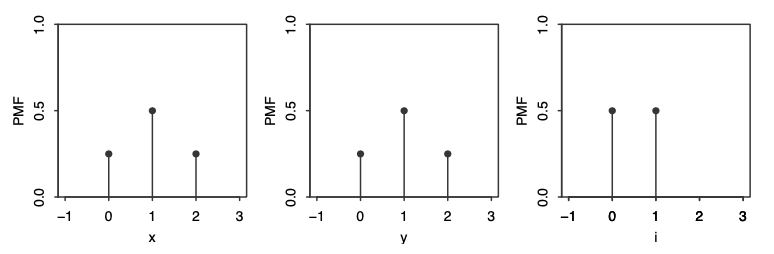
\includegraphics[width=1\linewidth]{figures/Picture07} 

}

\caption{Minh hoạ cho hàm khối xác suất}\label{fig:unnamed-chunk-5}
\end{figure}

\hypertarget{vuxed-dux1ee5-2}{%
\subsubsection{Ví dụ:}\label{vuxed-dux1ee5-2}}

Tung 2 xúc sắc \(A\) và \(B\). Xác định PMF của các biến số ngẫu nhiên sau:

\begin{itemize}
\tightlist
\item
  \(X\) là điểm số của xúc sắc \(A\).
\item
  \(Y\) là điểm số của xúc sắc \(B\)
\item
  \(Z = 7 - X\)
\item
  \(T = X + Y\)
\end{itemize}

PMF của \(T\) được minh hoạ trong hình sau:

\begin{figure}

{\centering 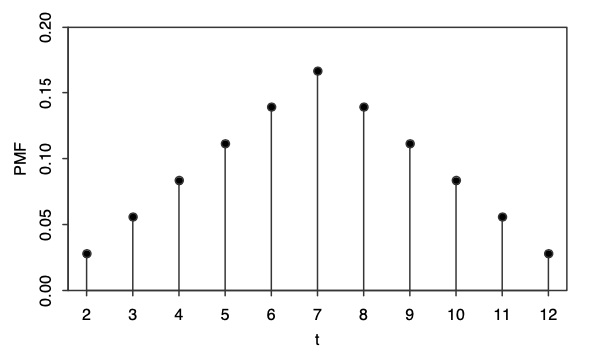
\includegraphics[width=1\linewidth]{figures/Picture08} 

}

\caption{Minh hoạ cho PMF của $T$}\label{fig:unnamed-chunk-6}
\end{figure}

\hypertarget{vuxed-dux1ee5-3}{%
\subsubsection{Ví dụ:}\label{vuxed-dux1ee5-3}}

Với ví dụ trên, tính xác suất tổng điểm của 2 xúc sắc (\(T\)) có giá trị từ 1 đến 4

\(P(1 \leq T \leq 4) = P(T = 2) + P(T = 3) + P(T = 4) = 6/36\)

\hypertarget{phuxe2n-phux1ed1i-bernoulli-bernoulli-distribution}{%
\subsubsection{Phân phối Bernoulli (Bernoulli distribution)}\label{phuxe2n-phux1ed1i-bernoulli-bernoulli-distribution}}

Một biến số ngẫu nhiên \(X\) có phân phối Bernoulli với tham số \(p\) nếu \(P(X = 1) = p\) và \(P(X = 0) = 1 - p\), với \(0 < p < 1\). Ta có thể ký hiệu là \(X \sim Bern(p)\)

Mọi biến số ngẫu nhiên chỉ có 2 giá trị \(0\) và \(1\) đều có phân phối Bernoulli với tham số \(p\) \(Bern(p)\), với \(p\) là xác suất biến số ngẫu nhiên có giá trị bằng \(1\).

\begin{quote}
Thử nghiệm Bernoulli (Bernoulli trial): Một thử nghiệm mà kết quả chỉ có 1 trong 2 kết cục: ``thành công'' hay ``thất bại'' được gọi là một thử nghiệm Bernoulli. Một biến số ngẫu nhiên Bernoulli có thể xem là chỉ tố của thành công trong một thử nghiệm Bernoulli.
\end{quote}

\hypertarget{phuxe2n-phux1ed1i-nhux1ecb-thux1ee9c-binomial-distribution}{%
\subsubsection{Phân phối nhị thức (Binomial distribution)}\label{phuxe2n-phux1ed1i-nhux1ecb-thux1ee9c-binomial-distribution}}

Thực hiện \(n\) thử nghiệm Bernoulli độc lập với nhau, mỗi thử nghiệm đều có xác suất thành công \(p\). Gọi \(X\) là tổng số lần thành công. Phân phối của \(X\) được gọi là phân phối nhị thức với các tham số là \(n\) và \(p\). Ta có thể ký hiệu là \(X \sim Bin(n, p)\)

Nếu \(X \sim Bin(n, p)\), PMF của \(X\) là

\[
P(X = k) = {n \choose k} p^k (1-p)^{n-k}
\]
Với \({n \choose k} = \frac{n!}{k!(n-k)!}\)

\begin{figure}

{\centering 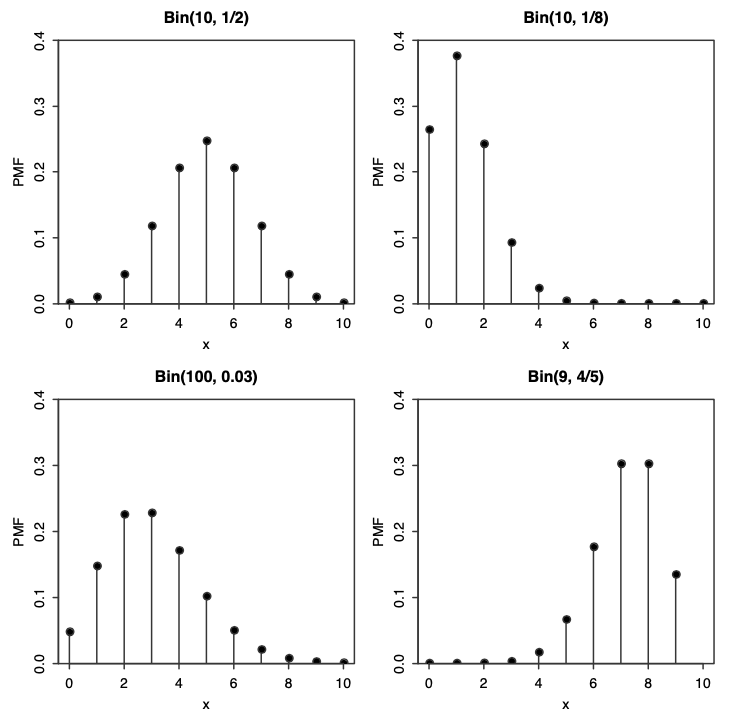
\includegraphics[width=1\linewidth]{figures/Picture09} 

}

\caption{Minh hoạ cho PMF của phân phối nhị thức}\label{fig:unnamed-chunk-7}
\end{figure}

\hypertarget{huxe0m-phuxe2n-phux1ed1i-tuxedch-luux1ef9-cumulative-distribution-functions-cdf}{%
\subsubsection{Hàm phân phối tích luỹ (Cumulative distribution functions, CDF)}\label{huxe0m-phuxe2n-phux1ed1i-tuxedch-luux1ef9-cumulative-distribution-functions-cdf}}

Hàm phân phối tích luỹ (CDF) của một biến số ngẫu nhiên \(X\) là một hàm số \(F_X\) với \(F_X(x) = P(X \leq x)\)

\hypertarget{tuxednh-chux1ea5t-cux1ee7a-cdf}{%
\subsubsection{Tính chất của CDF}\label{tuxednh-chux1ea5t-cux1ee7a-cdf}}

Bất kỳ hàm phân phối tích luỹ nào cũng có các tính chất sau:

\begin{itemize}
\tightlist
\item
  Tăng dần: nếu \(x_1 \leq x_2\) thì \(F(x_1) \leq F(x_2)\)
\item
  Có giới hạn là \(0\) và \(1\): \(\lim_{x\rightarrow -\infty}F(x) = 0\) và \(\lim_{x\rightarrow +\infty}F(x) = 1\)
\end{itemize}

Hình dưới đây minh hoạ cho PMF và CDF của phân phối \(Bin(4, 1/2)\)

\begin{figure}

{\centering 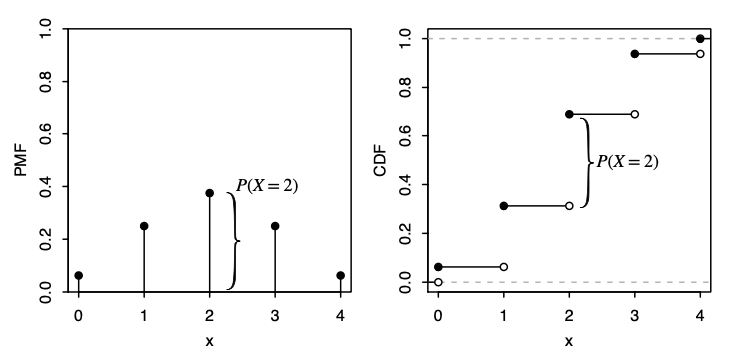
\includegraphics[width=1\linewidth]{figures/Picture10} 

}

\caption{Minh hoạ cho PMF của phân phối nhị thức}\label{fig:unnamed-chunk-8}
\end{figure}

\hypertarget{kuxec-vux1ecdng-expectation}{%
\subsubsection{Kì vọng (Expectation)}\label{kuxec-vux1ecdng-expectation}}

Kì vọng giúp tóm tắt phân phối của biến số ngẫu nhiên. Có 2 loại kì vọng chính:

\begin{itemize}
\tightlist
\item
  Vọng trị (Expected value): mô tả vị trí trung tâm của phân phối
\item
  Phương sai (Variance): mô tả độ phân tán của phân phối
\end{itemize}

Vọng trị (expected value) của một biến số ngẫu nhiên rời rạc \(X\) với các giá trị có thể có \(x_1, x_2, \ldots\) được định nghĩa như sau:

\[
E(X) = \Sigma^\infty_{j = 1} x_j P(X = x_j)
\]
Một số tính chất của vọng trị

\begin{itemize}
\tightlist
\item
  Với mọi biến số ngẫu nhiên \(X\), \(Y\) và hằng số \(c\): \(E(X + Y) = E(X) + E(Y)\) và \(E(cX) = c E(X)\)
\end{itemize}

Vọng trị của phân phối Bernoulli: Nếu \(X \sim Bern(p)\) thì \(E(X) = p\)

Vọng trị của phân phối nhị thức: Nếu \(X \sim Bin(n, p)\) thì \(E(X) = np\)

Phương sai (variance) và độ lệch chuẩn (standard deviation) của một biến số ngẫu nhiên X được định nghĩa như sau:

\[
Var(X) = E(X - EX)^2 = E(X^2) - (EX)^2
\]
\[
SD(X) = \sqrt{Var(X)}
\]
Phương sai của \(X\) đo lường trung bình bình phương khoảng cách trung bình từ các giá trị của \(X\) đến giá trị trung bình.

Các tính chất của phương sai:

\begin{itemize}
\tightlist
\item
  \(Var(X + c) = Var(X)\)
\item
  \(Var(cX) = c^2 Var(X)\)
\item
  Nếu \(X\) và \(Y\) độc lập, \(Var(X + Y) = Var(X) + Var(Y)\)
\end{itemize}

Phương sai của phân phối Bernoulli: Nếu \(X \sim Bern(p)\) thì \(Var(X) = p(1-p)\)

Phương sai của phân phối nhị thức: Nếu \(X \sim Bin(n, p)\) thì \(Var(X) = np(1-p)\)

\hypertarget{phuxe2n-phux1ed1i-cux1ee7a-biux1ebfn-sux1ed1-ngux1eabu-nhiuxean-liuxean-tux1ee5c}{%
\subsection{Phân phối của biến số ngẫu nhiên liên tục}\label{phuxe2n-phux1ed1i-cux1ee7a-biux1ebfn-sux1ed1-ngux1eabu-nhiuxean-liuxean-tux1ee5c}}

\hypertarget{huxe0m-mux1eadt-ux111ux1ed9-xuxe1c-suux1ea5t-probability-density-function-pdf.}{%
\subsubsection{Hàm mật độ xác suất (Probability density function, PDF).}\label{huxe0m-mux1eadt-ux111ux1ed9-xuxe1c-suux1ea5t-probability-density-function-pdf.}}

Với biến số ngẫu nhiên \(X\) có CDF \(F\), hàm mật độ xác suất (PDF) của \(X\) là đạo hàm \(f\) của CDF: \(f(x) = F^\prime(x)\)

Lưu ý, giá trị \(f(x)\) của PDF không phải là một xác suất (\(f(x)\) có thể \(>1\))

Chuyển đổi từ PDF sang CDF: \(X\) là biến số ngẫu nhiên với PDF \(f\). Khi đó CDF của \(X\) có thể được tính bằng:

\[
F(x) = \int^x_{-\infty} f(t)dt
\]
và xác suất \(X\) nằm trong khoảng từ \(a\) đến \(b\) có thể được tính theo công thức

\[
P(a < X \leq b) = \int^b_{a} f(x)dx
\]
Một số tính chất của PDF

\begin{itemize}
\tightlist
\item
  Không âm: \(f(x) \geq 0\)
\item
  Có tích phân bằng 1: \(\int_{-\infty}^{\infty}f(x)dx = 1\)
\end{itemize}

Vọng trị của một biến số ngẫu nhiên \(X\) có PDF \(f\) là

\[
E(X) = \int_{-\infty}^{\infty} xf(x)dx
\]
\#\#\#\# Phân phối chuẩn tắc (standard normal distribution)

Một biến số ngẫu nhiên \(Z\) có phân phối chuẩn tắc nếu có PDF

\[
\varphi(z) = \frac{1}{\sqrt{2\pi}}\exp^{-z^2/2}, -\infty < z < \infty
\]
\(Z\) có trung bình là \(0\) và phương sai là \(1\). Ta có thể ký hiệu: \(Z \sim N(0, 1)\)

\hypertarget{phuxe2n-phux1ed1i-buxecnh-thux1b0ux1eddng-normal-distribution}{%
\subsubsection{Phân phối bình thường (normal distribution)}\label{phuxe2n-phux1ed1i-buxecnh-thux1b0ux1eddng-normal-distribution}}

Một biến số ngẫu nhiên \(Z\) có phân phối chuẩn tắc (\(Z \sim N(0, 1)\)) thì

\[
X = \mu + \sigma Z
\]
có phân phối bình thường với trung bình \(\mu\) và phương sai \(\sigma^2\). Ta có thể ký hiệu là \(X \sim N(\mu, \sigma^2)\)

\hypertarget{ux1ee9ng-dux1ee5ng-cux1ee7a-xuxe1c-suux1ea5t-trong-chux1ea9n-ux111ouxe1n-vuxe0-ra-quyux1ebft-ux111ux1ecbnh-luxe2m-suxe0ng}{%
\section{Ứng dụng của xác suất trong chẩn đoán và ra quyết định lâm sàng}\label{ux1ee9ng-dux1ee5ng-cux1ee7a-xuxe1c-suux1ea5t-trong-chux1ea9n-ux111ouxe1n-vuxe0-ra-quyux1ebft-ux111ux1ecbnh-luxe2m-suxe0ng}}

\hypertarget{stkcb_thongke}{%
\chapter{Kiến thức cơ bản về thống kê y sinh}\label{stkcb_thongke}}

\hypertarget{part-muxf4-huxecnh-tiuxean-lux1b0ux1ee3ng-luxe2m-suxe0ng}{%
\part{MÔ HÌNH TIÊN LƯỢNG LÂM SÀNG}\label{part-muxf4-huxecnh-tiuxean-lux1b0ux1ee3ng-luxe2m-suxe0ng}}

\hypertarget{part-muxf4-huxecnh-touxe1n-hux1ecdc-trong-dux1ecbch-tux1ec5-hux1ecdc}{%
\part{MÔ HÌNH TOÁN HỌC TRONG DỊCH TỄ HỌC}\label{part-muxf4-huxecnh-touxe1n-hux1ecdc-trong-dux1ecbch-tux1ec5-hux1ecdc}}

\hypertarget{mhth_gioithieu}{%
\chapter{Giới thiệu về mô hình toán học trong dịch tễ học bệnh truyền nhiễm}\label{mhth_gioithieu}}

\hypertarget{mhth_khainiem}{%
\chapter{Các khái niệm cơ bản trong dịch tễ học bệnh truyền nhiễm}\label{mhth_khainiem}}

\hypertarget{mhth_buoc}{%
\chapter{Các bước cơ bản để xây dựng và đánh giá mô hình toán học trong dịch tễ học bệnh truyền nhiễm}\label{mhth_buoc}}

\hypertarget{mhth_congcu}{%
\chapter{Công cụ xây dựng và đánh giá mô hình toán học trong dịch tễ học bệnh truyền nhiễm với phần mềm R}\label{mhth_congcu}}

\hypertarget{mhth_thietke}{%
\chapter{Thiết kế mô hình}\label{mhth_thietke}}

\hypertarget{mhth_phuongphap}{%
\chapter{Lựa chọn phương pháp xây dựng mô hình}\label{mhth_phuongphap}}

\hypertarget{mhth_uoctinh}{%
\chapter{Ước tính tham số và độ bất định}\label{mhth_uoctinh}}

\hypertarget{mhth_giatri}{%
\chapter{Đánh giá tính giá trị của mô hình}\label{mhth_giatri}}

\hypertarget{mhth_trinhbay}{%
\chapter{Trình bày và công bố kết quả nghiên cứu dựa trên mô hình toán học}\label{mhth_trinhbay}}

\hypertarget{mhth_danhgiadich}{%
\chapter{Đánh giá tình hình dịch bằng mô hình toán học}\label{mhth_danhgiadich}}

\hypertarget{mhth_hieuquacanthiep}{%
\chapter{Đánh giá hiệu quả can thiệp bằng mô hình toán học}\label{mhth_hieuquacanthiep}}

\hypertarget{BayesDisTransModels}{%
\chapter{Xây dựng mô hình bệnh truyền nhiễm theo trường phái Bayes}\label{BayesDisTransModels}}

(dựa trên \citep{grinsztajn_bayesian_2021})

\hypertarget{muxf4-huxecnh-touxe1n-hux1ecdc-bux1ec7nh-truyux1ec1n-nhiux1ec5m}{%
\section{Mô hình toán học bệnh truyền nhiễm}\label{muxf4-huxecnh-touxe1n-hux1ecdc-bux1ec7nh-truyux1ec1n-nhiux1ec5m}}

Mô hình toán học bệnh truyền nhiễm giúp

\begin{itemize}
\tightlist
\item
  Đánh giá hiệu quả của các biện pháp can thiệp trên sự lây nhiễm
\item
  Đánh giá gánh nặng/ảnh hưởng của dịch bệnh
\item
  Ước tính tỉ lệ tử vong sau khi hiệu chỉnh cho sai lệch báo cáo
\end{itemize}

Mô hình có thể ở nhiều quy mô khác nhau:

\begin{itemize}
\tightlist
\item
  Quy mô cá thể: agent-based models
\item
  Quy mô dân số: compartmental models
\end{itemize}

Mô hình tại quy mô dân số bao gồm

\begin{itemize}
\tightlist
\item
  Deterministic models: ODEs
\item
  Stochastic models: simulation
\end{itemize}

\hypertarget{cuxe1c-bux1b0ux1edbc-xuxe2y-dux1ef1ng-muxf4-huxecnh}{%
\subsection{Các bước xây dựng mô hình}\label{cuxe1c-bux1b0ux1edbc-xuxe2y-dux1ef1ng-muxf4-huxecnh}}

\begin{figure}

{\centering 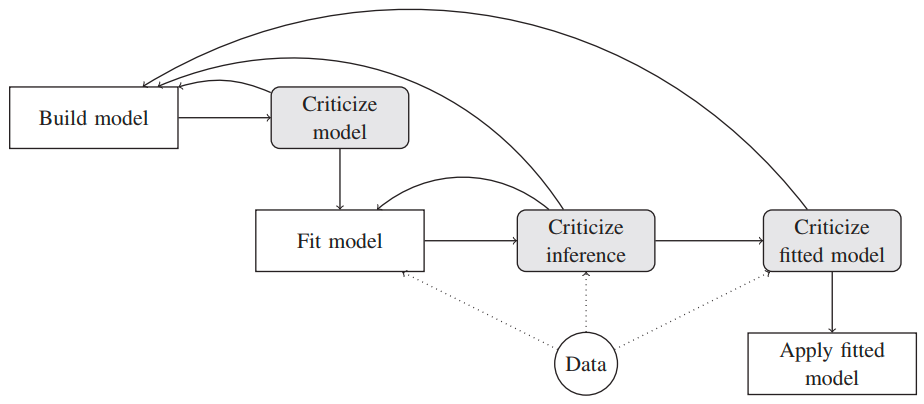
\includegraphics[width=1\linewidth]{figures/BayesDisTransModels_02} 

}

\caption{Các bước xây dựng mô hình}\label{fig:unnamed-chunk-9}
\end{figure}

\hypertarget{stan}{%
\section{Stan}\label{stan}}

\begin{figure}

{\centering 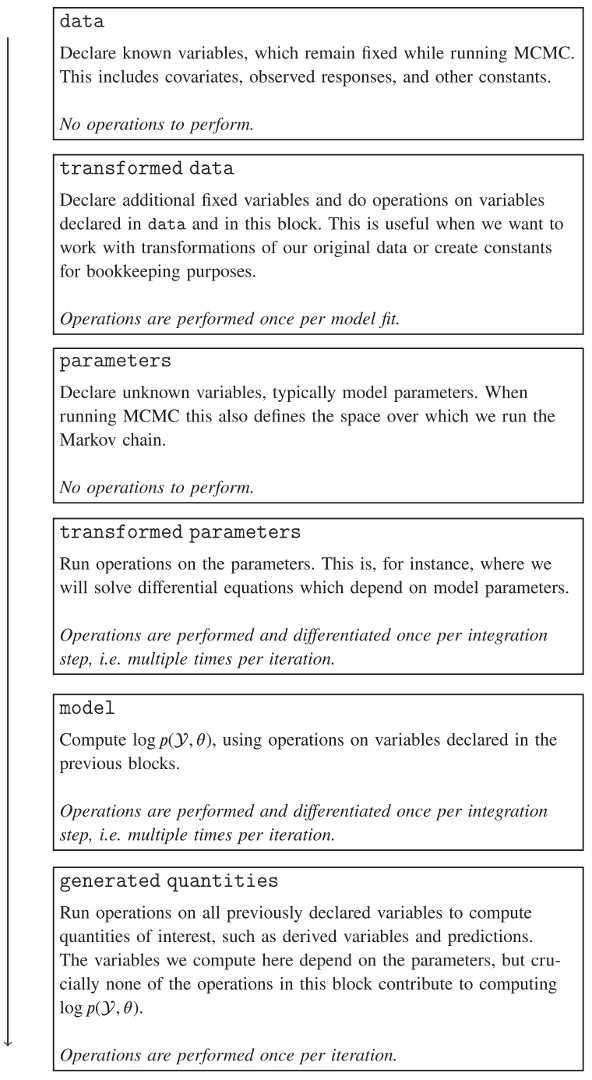
\includegraphics[width=1\linewidth]{figures/BayesDisTransModels_01} 

}

\caption{Cấu trúc code trong Stan}\label{fig:unnamed-chunk-10}
\end{figure}

\hypertarget{vuxed-dux1ee5-1-dux1ecbch-cuxfam-tux1ea1i-mux1ed9t-trux1b0ux1eddng-nux1ed9i-truxfa-ux1edf-anh-nux103m-1978}{%
\section{Ví dụ 1: dịch cúm tại một trường nội trú ở Anh năm 1978}\label{vuxed-dux1ee5-1-dux1ecbch-cuxfam-tux1ea1i-mux1ed9t-trux1b0ux1eddng-nux1ed9i-truxfa-ux1edf-anh-nux103m-1978}}

\hypertarget{bux1b0ux1edbc-1-xuxe2y-dux1ef1ng-muxf4-huxecnh}{%
\subsection{Bước 1: xây dựng mô hình}\label{bux1b0ux1edbc-1-xuxe2y-dux1ef1ng-muxf4-huxecnh}}

Mathematical transmission model:

\begin{itemize}
\tightlist
\item
  Mô hình SIR:

  \begin{itemize}
  \tightlist
  \item
    Tại thời điểm \(t\), số người cảm nhiễm (chưa có miễn dịch) là \(S(t)\), số người đang nhiễm bệnh và có khả năng lây bệnh là \(I(t)\), số người hồi phục là \(R(t)\) (có miễn dịch suốt đời).
  \item
    Xác suất để 1 người cảm nhiễm bị nhiễm bệnh là
  \end{itemize}

  \[ (\text{Số tiếp xúc} \times \text{Xác suất bị nhiễm bệnh khi tiếp xúc} \times \text{Xác suất tiếp xúc với người bị nhiễm bệnh})\]
  \[ \beta \times \dfrac{I(t)}{S(t)}\]

  \begin{itemize}
  \tightlist
  \item
    \(\beta\): tỉ suất lây truyền, transmission rate or effective contact rate (\(\text{Số tiếp xúc trong 1 đơn vị thời gian} \times \text{Xác suất bị nhiễm bệnh khi tiếp xúc với người bị nhiễm bệnh}\))

    \begin{itemize}
    \tightlist
    \item
      Tỉ suất tiếp xúc (contact rate): số tiếp xúc trong 1 đơn vị thời gian
    \item
      Nguy cơ lây nhiễm (transmission risk)
    \end{itemize}
  \item
    Giả định:

    \begin{itemize}
    \tightlist
    \item
      constant population
    \item
      indefinitely immune
    \item
      no incubation period
    \item
      Thời gian tại \(I\) \(\sim exp(1/\gamma)\)
    \item
      constant transmission rate \& recovery rate
    \item
      homogeneous mixing
    \end{itemize}
  \end{itemize}
\item
  Mô hình truyền nhiễm xác suất:

  \begin{itemize}
  \tightlist
  \item
    Likelihood: Số lượng BN quan sát được tại thời điểm \(t\) \(\sim \text{Negative Binomial}(I(t), \phi)\)
  \item
    Phân phối tiền nghiệm của các tham số:

    \begin{itemize}
    \tightlist
    \item
      Tỉ suất lây nhiễm \(\beta\): \(\text{Normal}^+(2, 1)\) (weakly informative prior, \(\beta\) dương {[}truncated at 0{]} \& soft higher limit around 4 {[}\(P(\beta < 4) = 0.975\){]})
    \item
      Tỉ suất hồi phục \(\gamma\): \(\text{Normal}^+(0.4, 0.5)\) (\(\gamma\) dương {[}truncated at 0{]} \& \(P(\gamma \leq 1) = 0.9\))
    \item
      Tham số dispersion: \(P(1/\phi) = \text{exponential}(5)\)
    \end{itemize}
  \end{itemize}
\end{itemize}

\hypertarget{bux1b0ux1edbc-2}{%
\subsection{Bước 2:}\label{bux1b0ux1edbc-2}}

\begin{Shaded}
\begin{Highlighting}[]
\CommentTok{\# library(rstan)}
\CommentTok{\# library(gridExtra)}
\CommentTok{\# rstan\_options(auto\_write = TRUE)}
\CommentTok{\# options(mc.cores = parallel::detectCores())}
\end{Highlighting}
\end{Shaded}

\begin{verbatim}
// functions block: specify ODEs
functions {
  real[] sir(real t, real[] y, real[] theta, 
             real[] x_r, int[] x_i) {

      real S = y[1];
      real I = y[2];
      real R = y[3];
      real N = x_i[1];
      
      real beta = theta[1];
      real gamma = theta[2];
      
      real dS_dt = -beta * I * S / N;
      real dI_dt =  beta * I * S / N - gamma * I;
      real dR_dt =  gamma * I;
      
      return {dS_dt, dI_dt, dR_dt};
  }
}

data {
  int<lower=1> n_days;
  real y0[3];
  real t0;
  real ts[n_days];
  int N;
  int cases[n_days];
}

transformed data {
  real x_r[0];
  int x_i[1] = { N };
}

parameters {
  real<lower=0> gamma;
  real<lower=0> beta;
  real<lower=0> phi_inv;
}

transformed parameters{
  real y[n_days, 3];
  real phi = 1. / phi_inv;
  {
    real theta[2];
    theta[1] = beta;
    theta[2] = gamma;

    y = integrate_ode_rk45(sir, y0, t0, ts, theta, x_r, x_i);
  }
}

model {
  //priors
  beta ~ normal(2, 1); //truncated at 0
  gamma ~ normal(0.4, 0.5); //truncated at 0
  phi_inv ~ exponential(5);
  
  //sampling distribution
  //col(matrix x, int n) - The n-th column of matrix x. Here the number of infected people
  cases ~ neg_binomial_2(col(to_matrix(y), 2), phi);
}

generated quantities {
  real R0 = beta / gamma;
  real recovery_time = 1 / gamma;
  real pred_cases[n_days];
  pred_cases = neg_binomial_2_rng(col(to_matrix(y), 2) + 1e-5, phi);
}
\end{verbatim}

\begin{Shaded}
\begin{Highlighting}[]
\CommentTok{\# \# time series of cases}
\CommentTok{\# library(outbreaks)}
\CommentTok{\# library(tidyverse)}
\CommentTok{\# cases \textless{}{-} influenza\_england\_1978\_school$in\_bed  \# Number of students in bed}
\CommentTok{\# }
\CommentTok{\# \# total count}
\CommentTok{\# N \textless{}{-} 763;}
\CommentTok{\# }
\CommentTok{\# \# times}
\CommentTok{\# n\_days \textless{}{-} length(cases) }
\CommentTok{\# t \textless{}{-} seq(0, n\_days, by = 1)}
\CommentTok{\# t0 \textless{}{-} 0 }
\CommentTok{\# t \textless{}{-} t[{-}1]}
\CommentTok{\# }
\CommentTok{\# \#initial conditions}
\CommentTok{\# i0 \textless{}{-} 1}
\CommentTok{\# s0 \textless{}{-} N {-} i0}
\CommentTok{\# r0 \textless{}{-} 0}
\CommentTok{\# y0 = c(S = s0, I = i0, R = r0)}
\CommentTok{\# }
\CommentTok{\# \# data for Stan}
\CommentTok{\# data\_sir \textless{}{-} list(n\_days = n\_days, y0 = y0, t0 = t0, ts = t, N = N, cases = cases, compute\_likelihood = 0)}
\CommentTok{\# }
\CommentTok{\# \# number of MCMC steps}
\CommentTok{\# niter \textless{}{-} 2000}
\end{Highlighting}
\end{Shaded}

\begin{Shaded}
\begin{Highlighting}[]
\CommentTok{\# set.seed(10)}
\CommentTok{\# model \textless{}{-} stan\_model(file.path("code", "BayesDisTransModels", "sir\_negbin.stan"))}
\CommentTok{\# fit\_sir\_negbin \textless{}{-} sampling(model,}
\CommentTok{\#                 data = data\_sir,}
\CommentTok{\#                 iter = niter,}
\CommentTok{\#                 chains = 4, }
\CommentTok{\#                 seed = 0)}
\end{Highlighting}
\end{Shaded}

\hypertarget{prior-predictive-check}{%
\section{prior predictive check}\label{prior-predictive-check}}

\hypertarget{part-kux1ef9-nux103ng}{%
\part{KỸ NĂNG}\label{part-kux1ef9-nux103ng}}

\hypertarget{kn_tltk}{%
\chapter{Tìm kiếm \& quản lý tài liệu tham khảo}\label{kn_tltk}}

\hypertarget{kn_tqyv}{%
\chapter{Tổng quan y văn}\label{kn_tqyv}}

\hypertarget{kn_ccttsl}{%
\chapter{Xây dựng công cụ thu thập số liệu}\label{kn_ccttsl}}

\hypertarget{part-hux1ed9i-nghux1ecb-khoa-hux1ecdc}{%
\part{HỘI NGHỊ KHOA HỌC}\label{part-hux1ed9i-nghux1ecb-khoa-hux1ecdc}}

\hypertarget{hn_iscb41}{%
\chapter{ISCB 41 (2020)}\label{hn_iscb41}}

\hypertarget{hn_iscb42}{%
\chapter{ISCB 42 (2021)}\label{hn_iscb42}}

\hypertarget{part-khouxe1-hux1ecdc-ngux1eafn-hux1ea1n}{%
\part{KHOÁ HỌC NGẮN HẠN}\label{part-khouxe1-hux1ecdc-ngux1eafn-hux1ea1n}}

  \bibliography{book.bib,packages.bib}

\end{document}
